% Document collecting the table of means and mechanisms tables
\documentclass{article}
\usepackage{booktabs}
\usepackage{siunitx}
\usepackage{makecell}
\usepackage{threeparttable}
\usepackage[normalem]{ulem}
\usepackage{float}
\usepackage{amsfonts}  % Minimal
\usepackage{amssymb}   % Includes amsfonts and more
\usepackage{amsmath}
% Additional packages for landscape pages
\usepackage{dsfont}
\usepackage{pdflscape}
\usepackage{tabularx}

\usepackage{tabularx,array}
\usepackage{graphicx}
% define a “centering” version of X
\newcolumntype{C}{>{\centering\arraybackslash}X}

%\setlength{\tabcolsep}{8pt}

% Base directory for cleaned results
\newcommand{\cleanedresultsdir}{../results/cleaned}
% Base directory for figures
\newcommand{\figdir}{../results/figures}

\begin{document}

% -------------------------------------------------------------------------
%  Figures – key descriptive plots
% -------------------------------------------------------------------------
\section{Figures}

\begin{figure}[H]
  \centering
  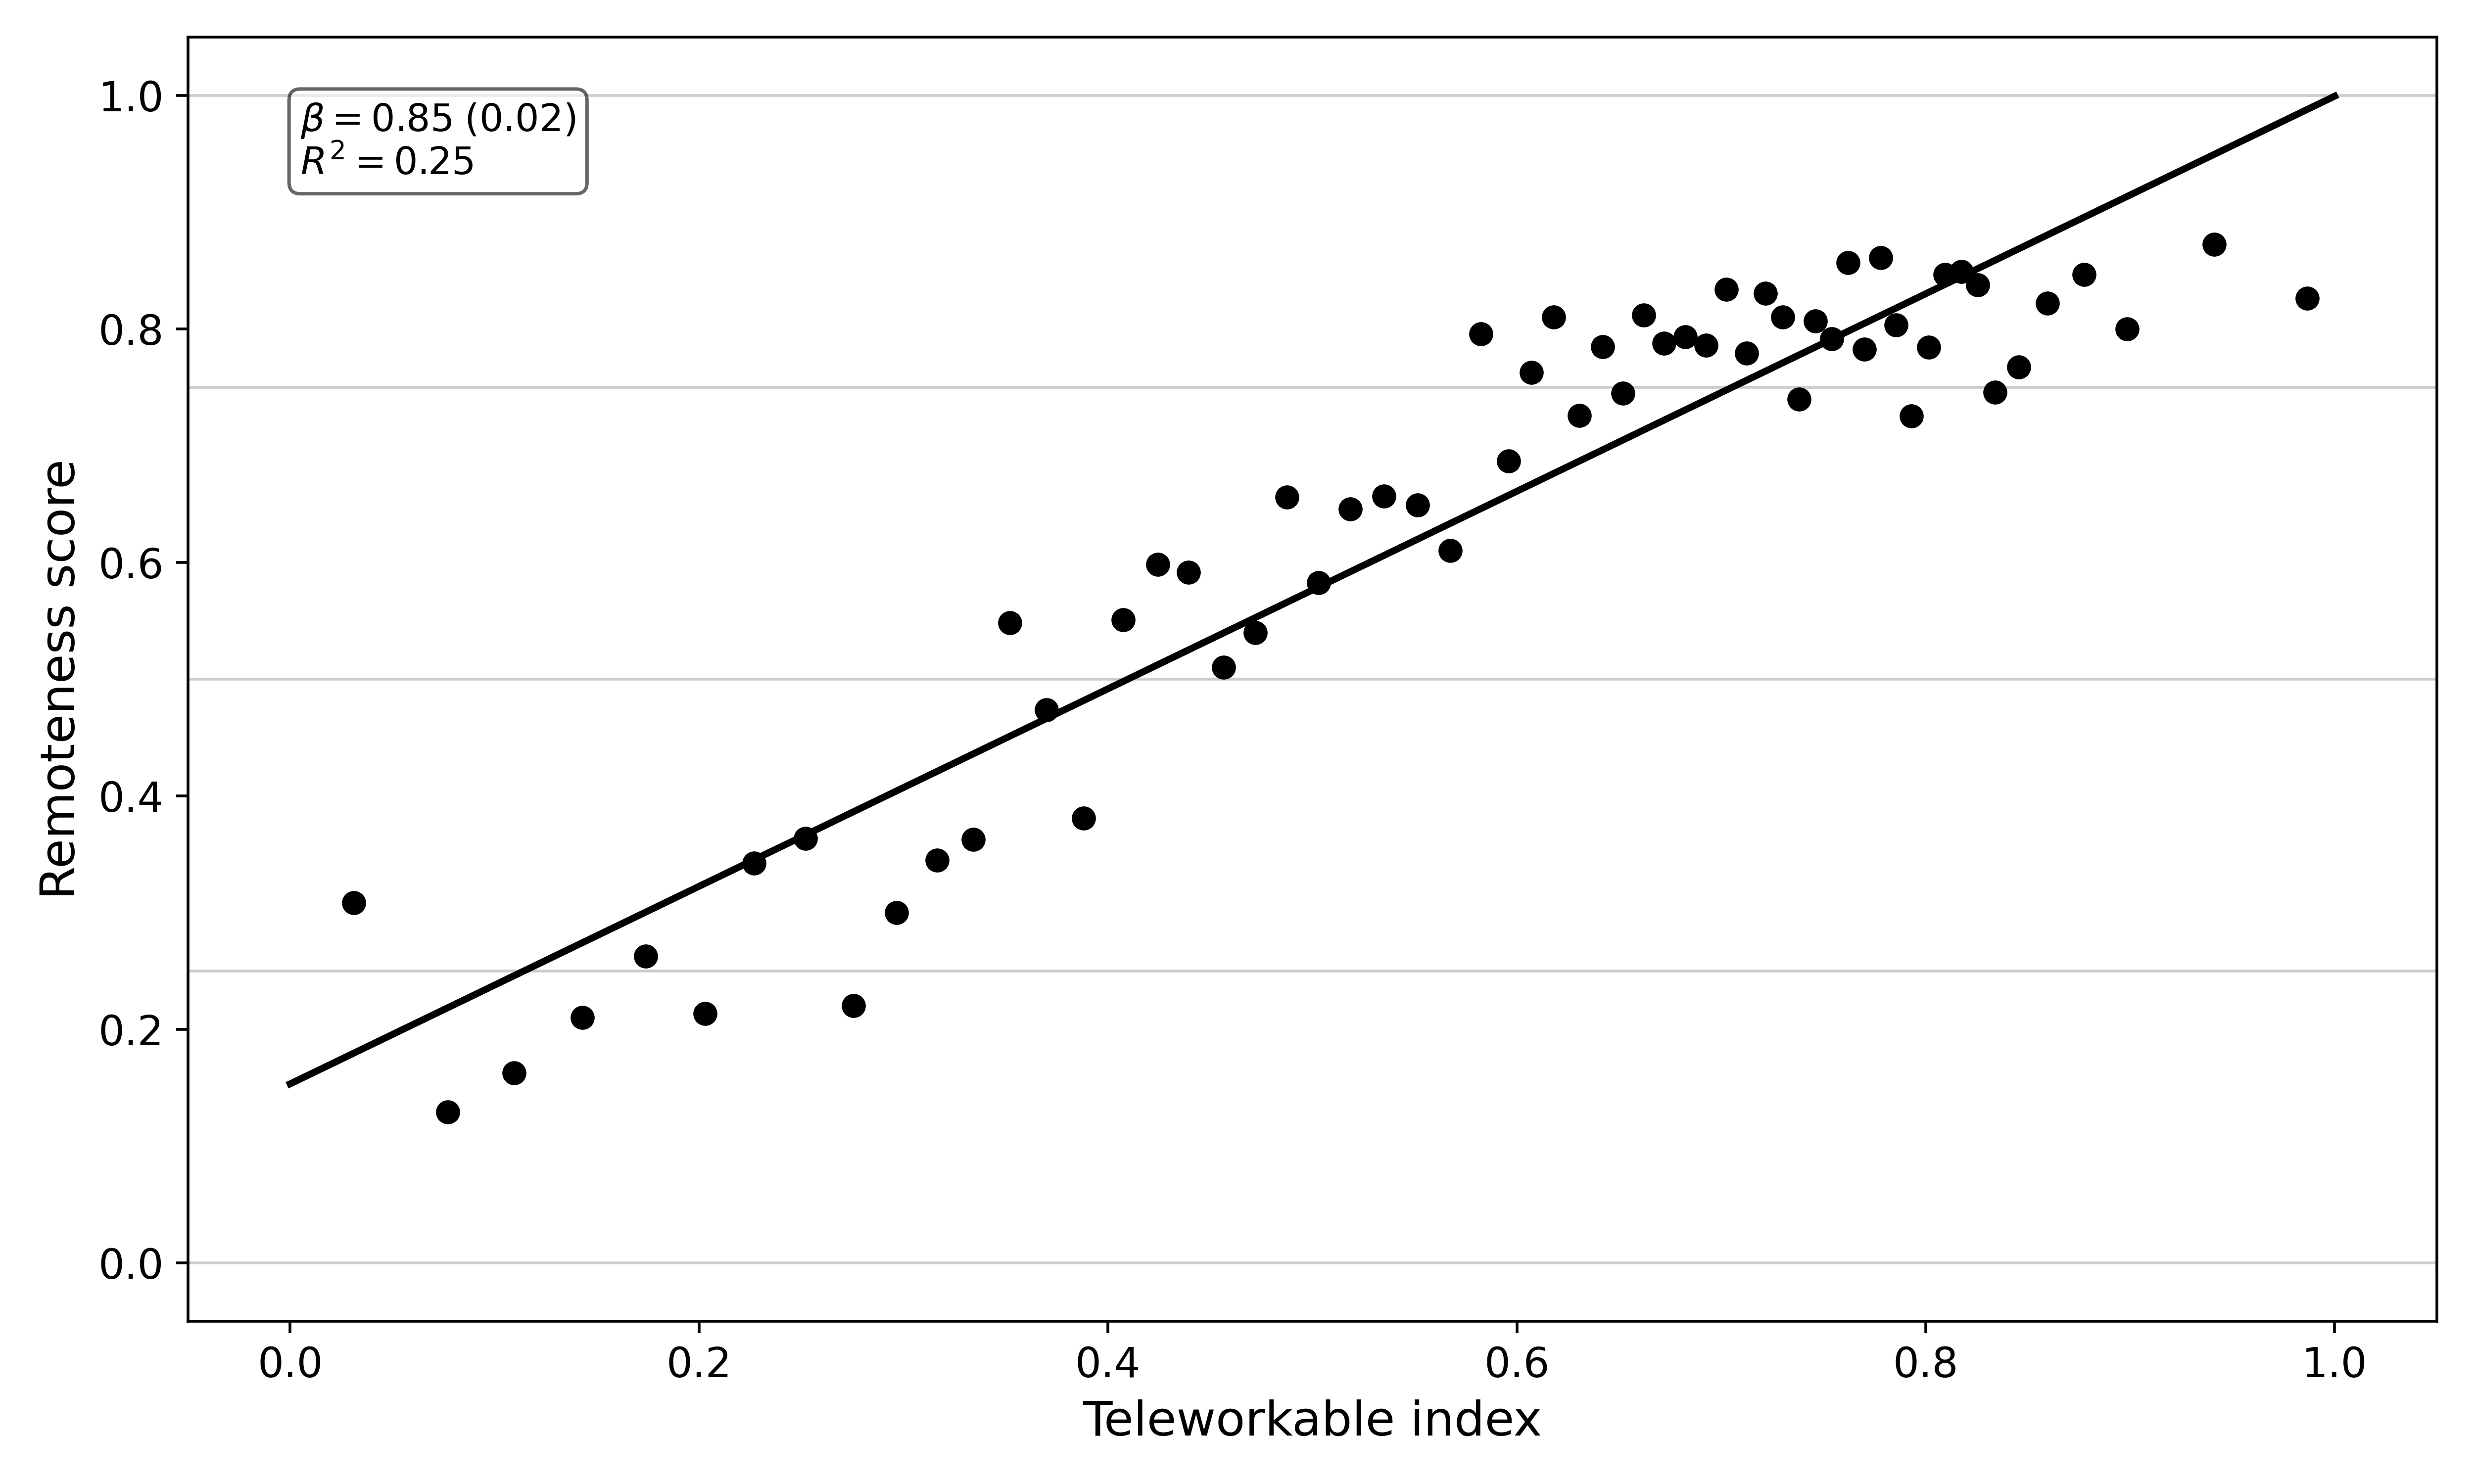
\includegraphics[width=0.9\textwidth]{\figdir/firm_teleworkable_remote.png}
  \caption{Remote v. Teleworkabe Scores}
\end{figure}

\begin{figure}[H]
  \centering
  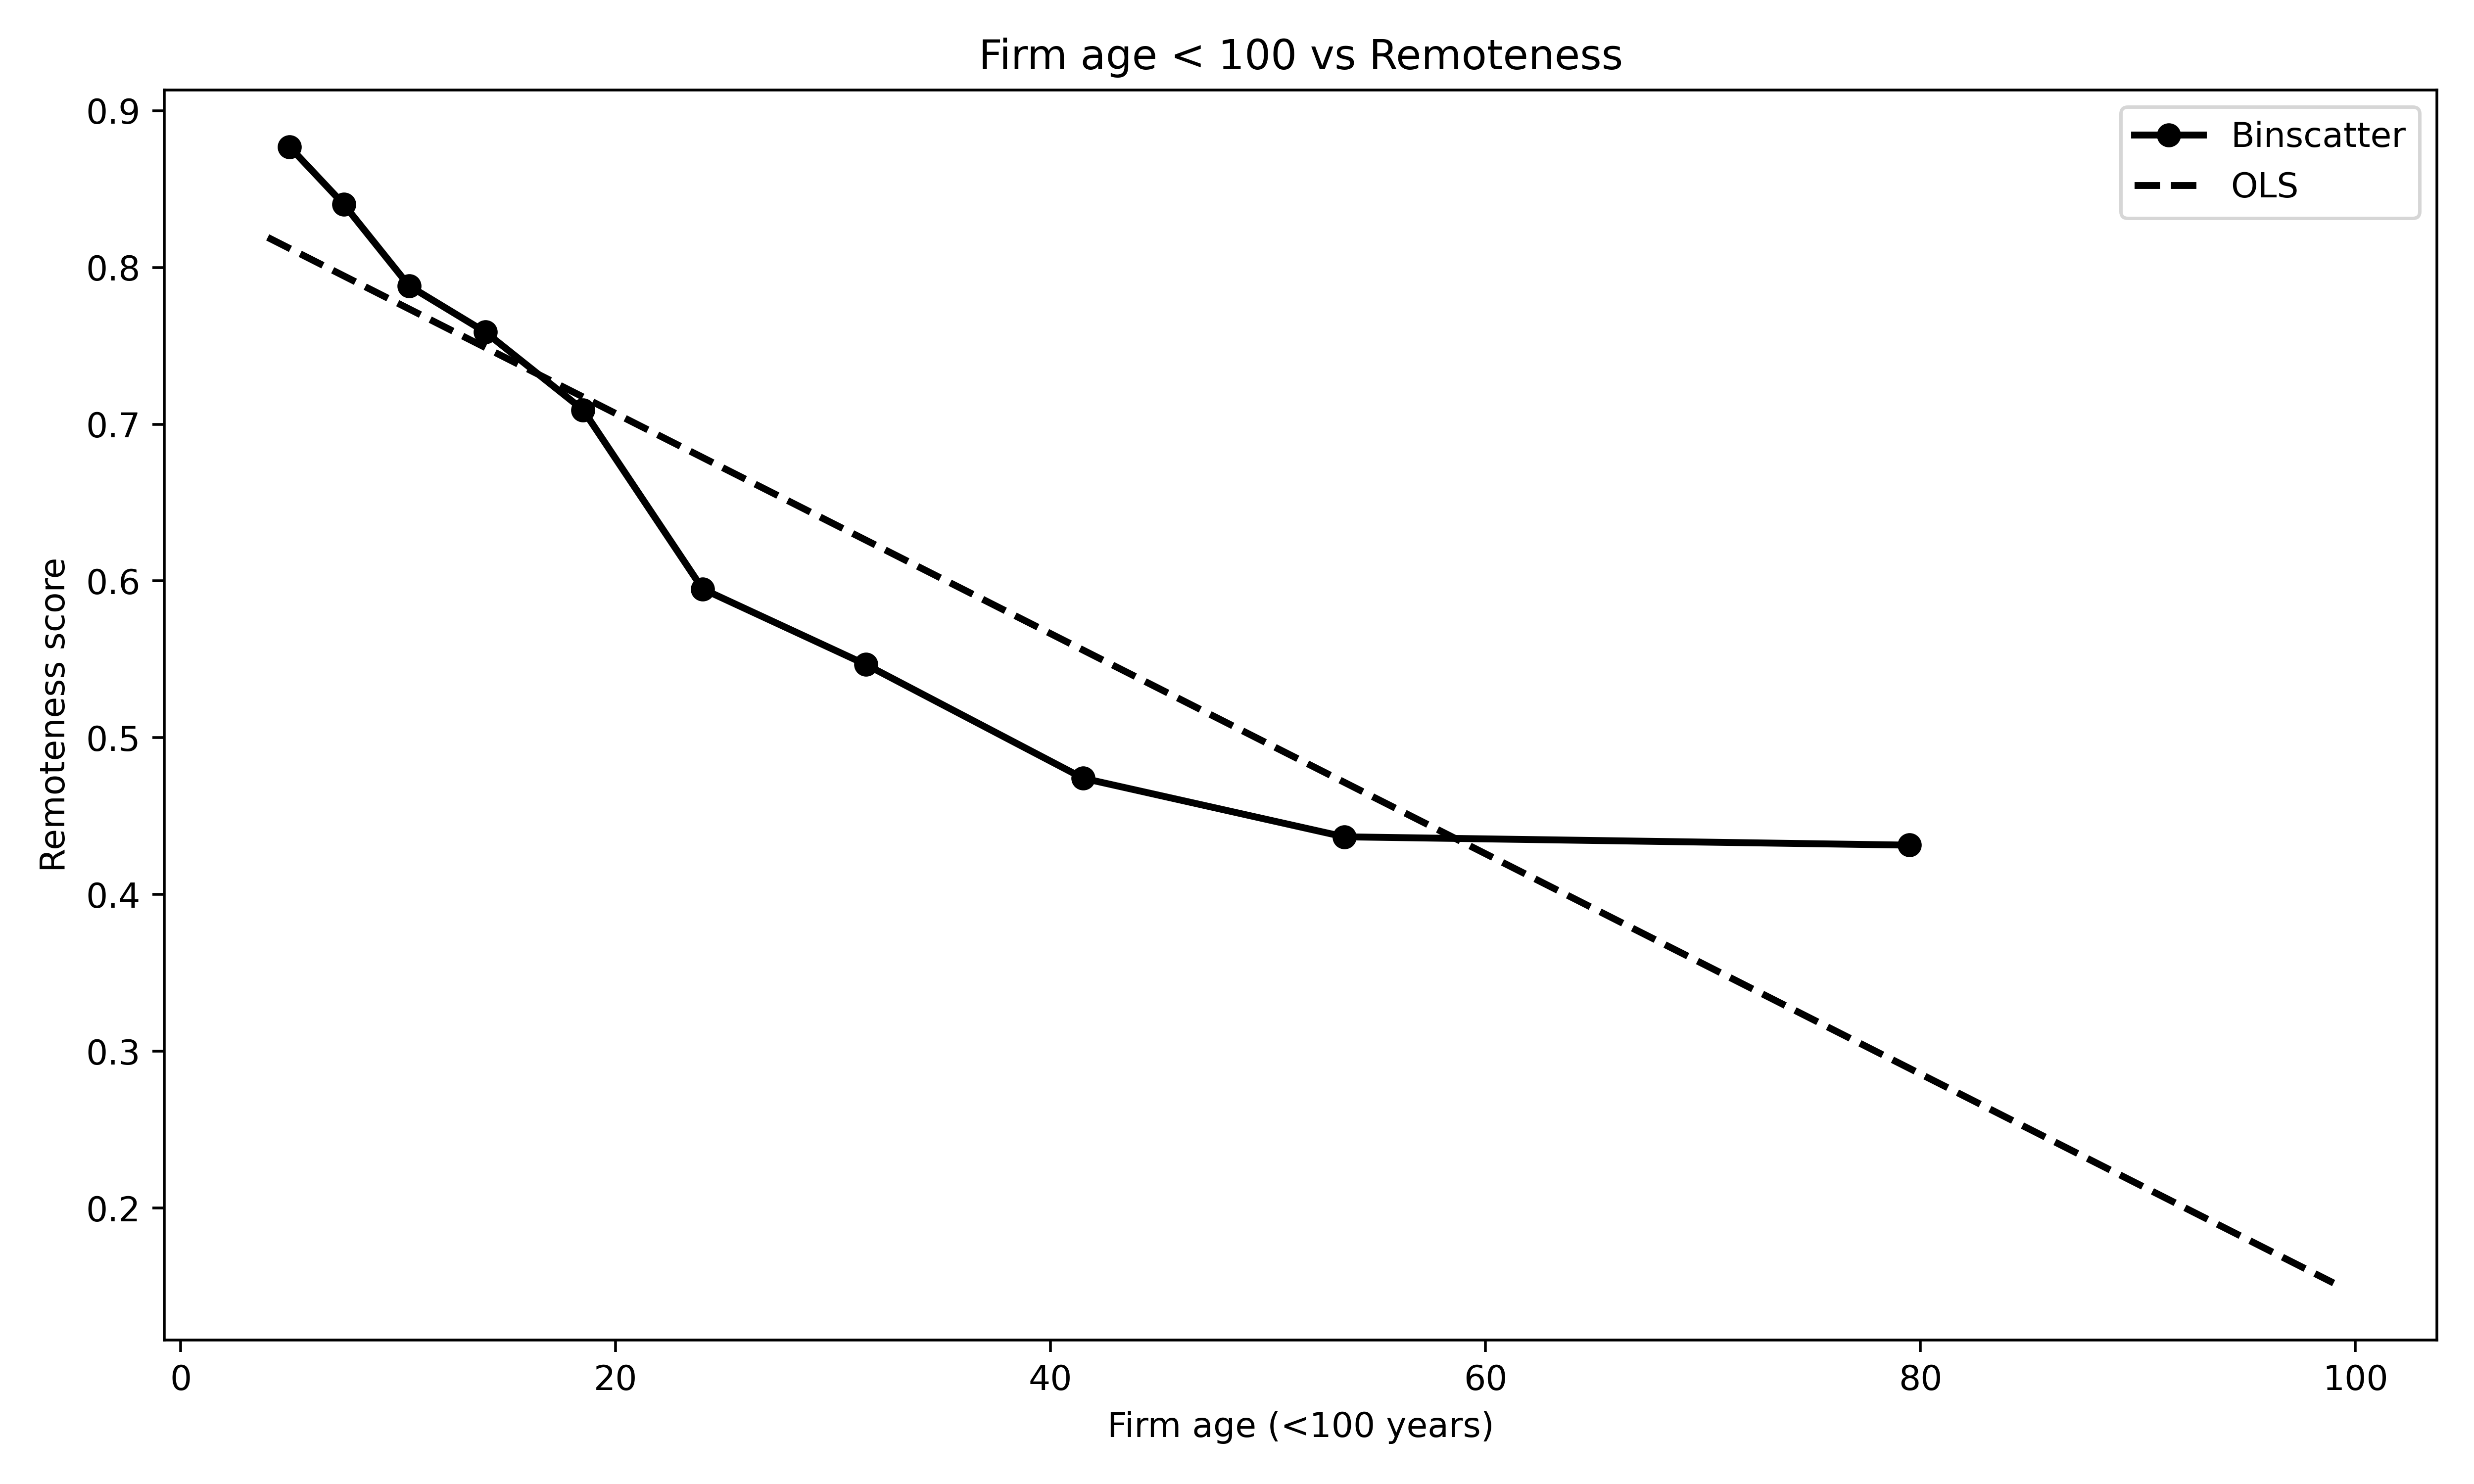
\includegraphics[width=0.9\textwidth]{\figdir/firm_age_lt100_remote.png}
  \caption{Remote v. Firm Age (\textless{} 100 employees)}
\end{figure}

\clearpage

\section{Table of Means}
\begin{table}[H]
        \centering
        \begin{threeparttable}
        \caption{Table of Means}
        \label{tab:means}
        \begin{tabular}{lcc@{\hspace{6pt}}c}
        \toprule
         & Startup & Incumbent & All Firms \\
        \midrule
        \addlinespace
        \multicolumn{4}{l}{\textbf{\uline{Panel A: Firm-level}}}\\[0.3em]
        Growth & \makecell{0.20 \\ (0.31)} & \makecell{0.06 \\ (0.16)} & \makecell{0.09 \\ (0.22)} \\
Leave & \makecell{0.26 \\ (0.31)} & \makecell{0.21 \\ (0.28)} & \makecell{0.22 \\ (0.29)} \\
Join & \makecell{0.35 \\ (0.32)} & \makecell{0.17 \\ (0.18)} & \makecell{0.22 \\ (0.24)} \\
Teleworkable Score \,(0--1) & \makecell{0.67 \\ (0.18)} & \makecell{0.54 \\ (0.25)} & \makecell{0.57 \\ (0.24)} \\
Remote Score \,(0--1) & \makecell{0.85 \\ (0.30)} & \makecell{0.57 \\ (0.41)} & \makecell{0.64 \\ (0.40)} \\
Employees (Count) & \makecell{271 \\ (1432)} & \makecell{2740 \\ (9555)} & \makecell{2126 \\ (8380)} \\
Age & \makecell{7 \\ (2)} & \makecell{43 \\ (34)} & \makecell{34 \\ (33)} \\
Rent (\textdollar/sq ft) & \makecell{49 \\ (21)} & \makecell{37 \\ (19)} & \makecell{40 \\ (20)} \\
Centrality Score & \makecell{1419 \\ (1830)} & \makecell{949 \\ (1309)} & \makecell{1066 \\ (1470)} \\
Seniority Levels (Count) & \makecell{3.62 \\ (0.77)} & \makecell{3.86 \\ (0.50)} & \makecell{3.80 \\ (0.59)} \\
\addlinespace
\midrule
Number of firms & 878 & 2630 & 3508 \\
Observations & 10450 & 31530 & 41980 \\
        \addlinespace
        \midrule
        \addlinespace
        \multicolumn{4}{l}{\textbf{\uline{Panel B: User-level}}}\\[0.3em]
        Total Contributions & \makecell{363.55 \\ (796.33)} & \makecell{193.43 \\ (641.42)} & \makecell{225.69 \\ (676.83)} \\
Restricted Contributions & \makecell{319.21 \\ (727.47)} & \makecell{138.68 \\ (356.21)} & \makecell{172.91 \\ (456.26)} \\
\addlinespace
\midrule
Number of firms & 727 & 1530 & 2257 \\
Number of users & 8635 & 33351 & 38411 \\
Observations & 48756 & 208390 & 257146 \\
        \bottomrule
        \end{tabular}
        \begin{tablenotes}[flushleft]
\footnotesize
\item \emph{Notes}: Panel~A uses firm--half--year observations. Panel~B relies on worker--half--year observations. ``Number of firms'' counts distinct firm\,IDs that ever appear in each category over the full sample window, so Startup and Incumbent counts need not sum to the ``All'' column. \textit{Growth}, \textit{Leave}, and \textit{Join} rates are fractions between 0 and 1. \textit{Teleworkable} and \textit{Remote} scores are index values between~0 and~1.  The sample period spans 2016 H2–2022 H1 at the firm level and 2017 H1–2022 H1 at the user level.
\end{tablenotes}
        \end{threeparttable}
        \end{table}


\section{Mechanisms}

We begin with the “base” specification:
\[
\begin{aligned}
y_{it} &= \alpha 
  + \beta_1\,(remote_i \times covid_t)
  + \beta_2\,(remote_i \times covid_t \times startup_i) \\
       &\quad
  + \delta\,(covid_t \times startup_i)
  + \mathrm{FE}_{it}
  + \varepsilon_{it},
\end{aligned}
\]
which captures how the outcome responds to remote work during COVID and
whether that effect differs in young firms.

In the \textbf{rent} “mirror” model we add two additional channels:
\[
\begin{aligned}
y_{it} &= \alpha 
  + \beta_1\,(remote_i \times covid_t)
  + \beta_2\,(remote_i \times covid_t \times startup_i) \\
       &\quad
  + \delta\,(covid_t \times startup_i)
  + \gamma_1\,(covid_t \times rent_i)
  + \gamma_2\,(remote_i \times covid_t \times rent_i) \\
       &\quad
  + \mathrm{FE}_{it}
  + \varepsilon_{it},
\end{aligned}
\]
so that \(\gamma_1\) and \(\gamma_2\) capture how both the baseline COVID
effect and the remote‐work premium vary with local office rents.

Likewise, the \textbf{centrality} (HHI) model adds:
\[
\begin{aligned}
y_{it} &= \alpha 
  + \beta_1\,(remote_i \times covid_t)
  + \beta_2\,(remote_i \times covid_t \times startup_i) \\
       &\quad
  + \delta\,(covid_t \times startup_i)
  + \gamma_1\,(covid_t \times hhi_i)
  + \gamma_2\,(remote_i \times covid_t \times hhi_i) \\
       &\quad
  + \mathrm{FE}_{it}
  + \varepsilon_{it}.
\end{aligned}
\]
By turning on each check‐mark (rent, centrality, seniority) one at a time—and
then in combination—we “mirror” the base COVID×Remote specification through
different mechanisms.



	\clearpage
	\begin{landscape}
	\subsection{User Productivity Mechanisms}
	\begin{table}[H]
\centering
\caption{User Productivity Mechanisms}
\begin{tabular}{lcccccccc}
\toprule
 & \multicolumn{8}{c}{Total Contributions} \\
\cmidrule(lr){2-9}
Specification & (1) & (2) & (3) & (4) & (5) & (6) & (7) & (8) \\
\midrule
Baseline & \checkmark & \checkmark & \checkmark & \checkmark & \checkmark & \checkmark & \checkmark & \checkmark \\
Rent &  & \checkmark &  & \checkmark &  & \checkmark &  & \checkmark \\
HHI &  &  & \checkmark & \checkmark &  &  & \checkmark & \checkmark \\
Seniority &  &  &  &  & \checkmark & \checkmark & \checkmark & \checkmark \\
\midrule
\multicolumn{9}{l}{\textbf{\uline{Panel A: OLS}}} \\
\addlinespace
$ \text{Remote} \times \mathds{1}(\text{Post}) $ & -2.66*** & 0.18 & -2.52* & 1.14 & 12.69 & 14.73 & 16.23 & 19.07 \\
 & (0.99) & (2.33) & (1.30) & (2.45) & (11.42) & (11.41) & (11.83) & (11.83) \\
$ \text{Remote} \times \mathds{1}(\text{Post}) \times \text{Startup} $ & 9.18*** & 8.50*** & 8.33*** & 8.47*** & 8.09*** & 7.93*** & 7.60*** & 7.75*** \\
 & (2.69) & (2.74) & (2.92) & (2.92) & (2.76) & (2.79) & (2.95) & (2.95) \\
\midrule
N & 52,995 & 51,392 & 51,392 & 51,392 & 51,392 & 51,392 & 51,392 & 51,392 \\
\multicolumn{9}{l}{\textbf{\uline{Panel B: IV}}} \\
\addlinespace
$ \text{Remote} \times \mathds{1}(\text{Post}) $ & -17.36** & -662.28 & 123.22 & -312.49 & -21312.51 & 160.32 & 957.68 & -267.63 \\
 & (8.72) & (1258.52) & (577.60) & (1438.40) & (66029.30) & (922.16) & (3030.76) & (3882.03) \\
$ \text{Remote} \times \mathds{1}(\text{Post}) \times \text{Startup} $ & 31.85*** & 117.04 & 211.08 & 238.68 & -47.81 & 70.47 & -107.21 & 227.12 \\
 & (12.28) & (170.78) & (709.68) & (398.71) & (427.16) & (66.79) & (379.62) & (1235.02) \\
\midrule
N & 52,995 & 47,771 & 47,771 & 47,771 & 47,771 & 47,771 & 47,771 & 47,771 \\
KP\,rk Wald F & 26.05 & 0.09 & 0.02 & 0.04 & 0.03 & 0.08 & 0.05 & 0.00 \\
\bottomrule
\end{tabular}
\label{tab:user_mechanisms}
\end{table}
	\end{landscape}

\clearpage
\begin{landscape}
\subsection{Firm Mechanisms}
\begin{table}[H]
\centering
\caption{Firm Mechanisms (Part 1)}
\begin{tabular}{lcccccccc}
\toprule
 & \multicolumn{8}{c}{Growth Rate} \\
\cmidrule(lr){2-9}
Specification & (1) & (2) & (3) & (4) & (5) & (6) & (7) & (8) \\
\midrule
Rent &  & \checkmark &  &  &  & \checkmark & \checkmark & \checkmark \\
Hhi &  &  & \checkmark &  &  & \checkmark &  &  \\
Seniority &  &  &  & \checkmark &  &  & \checkmark &  \\
Wage &  &  &  &  & \checkmark &  &  & \checkmark \\
\midrule
\multicolumn{9}{l}{\textbf{\uline{Panel A: OLS}}} \\
\addlinespace
$ \text{Remote} \times \mathds{1}(\text{Post}) $ & 0.001 & 0.007 & -0.019*** & 0.024 & -0.041*** & -0.016 & 0.028 & -0.035** \\
 & (0.005) & (0.011) & (0.007) & (0.024) & (0.012) & (0.013) & (0.026) & (0.015) \\
$ \text{Remote} \times \mathds{1}(\text{Post}) \times \text{Startup} $ & 0.070*** & 0.071*** & 0.063** & 0.068*** & 0.066*** & 0.063** & 0.068*** & 0.066*** \\
 & (0.025) & (0.026) & (0.025) & (0.025) & (0.025) & (0.025) & (0.025) & (0.026) \\
\midrule
N & 38,436 & 38,436 & 38,436 & 38,436 & 38,436 & 38,436 & 38,436 & 38,436 \\
\midrule
\multicolumn{9}{l}{\textbf{\uline{Panel B: IV}}} \\
\addlinespace
$ \text{Remote} \times \mathds{1}(\text{Post}) $ & 0.010 & -0.113*** & -0.039** & -0.037 & -0.042 & -0.157*** & -0.150* & -0.153*** \\
 & (0.009) & (0.043) & (0.018) & (0.067) & (0.028) & (0.044) & (0.079) & (0.048) \\
$ \text{Remote} \times \mathds{1}(\text{Post}) \times \text{Startup} $ & 0.157 & 0.139 & 0.037 & 0.122 & 0.149 & 0.026 & 0.109 & 0.133 \\
 & (0.100) & (0.099) & (0.102) & (0.096) & (0.100) & (0.101) & (0.096) & (0.099) \\
\midrule
N & 38,436 & 38,436 & 38,436 & 38,436 & 38,436 & 38,436 & 38,436 & 38,436 \\
KP\,rk Wald F & 14.56 & 11.27 & 10.14 & 9.84 & 9.56 & 8.41 & 8.35 & 8.15 \\
\bottomrule
\end{tabular}
\label{tab:firm_mechanisms_1}
\end{table}

\begin{table}[H]
\centering
\caption{Firm Mechanisms (Part 2)}
\begin{tabular}{lcccccccc}
\toprule
 & \multicolumn{8}{c}{Growth Rate} \\
\cmidrule(lr){2-9}
Specification & (1) & (2) & (3) & (4) & (5) & (6) & (7) & (8) \\
\midrule
Rent &  &  &  & \checkmark & \checkmark & \checkmark &  & \checkmark \\
Hhi & \checkmark & \checkmark &  & \checkmark & \checkmark &  & \checkmark & \checkmark \\
Seniority & \checkmark &  & \checkmark & \checkmark &  & \checkmark & \checkmark & \checkmark \\
Wage &  & \checkmark & \checkmark &  & \checkmark & \checkmark & \checkmark & \checkmark \\
\midrule
\multicolumn{9}{l}{\textbf{\uline{Panel A: OLS}}} \\
\addlinespace
$ \text{Remote} \times \mathds{1}(\text{Post}) $ & -0.022 & -0.053*** & -0.016 & -0.019 & -0.050*** & -0.011 & -0.055** & -0.052* \\
 & (0.026) & (0.012) & (0.026) & (0.029) & (0.016) & (0.027) & (0.028) & (0.030) \\
$ \text{Remote} \times \mathds{1}(\text{Post}) \times \text{Startup} $ & 0.064*** & 0.059** & 0.064*** & 0.065** & 0.059** & 0.064** & 0.061** & 0.061** \\
 & (0.025) & (0.025) & (0.025) & (0.025) & (0.025) & (0.025) & (0.025) & (0.025) \\
\midrule
N & 38,436 & 38,436 & 38,436 & 38,436 & 38,436 & 38,436 & 38,436 & 38,436 \\
\midrule
\multicolumn{9}{l}{\textbf{\uline{Panel B: IV}}} \\
\addlinespace
$ \text{Remote} \times \mathds{1}(\text{Post}) $ & -0.159** & -0.061* & -0.083 & -0.270*** & -0.169*** & -0.184** & -0.174** & -0.275*** \\
 & (0.072) & (0.033) & (0.068) & (0.083) & (0.049) & (0.078) & (0.072) & (0.081) \\
$ \text{Remote} \times \mathds{1}(\text{Post}) \times \text{Startup} $ & 0.056 & 0.038 & 0.116 & 0.045 & 0.028 & 0.104 & 0.058 & 0.048 \\
 & (0.101) & (0.101) & (0.097) & (0.100) & (0.100) & (0.096) & (0.101) & (0.100) \\
\midrule
N & 38,436 & 38,436 & 38,436 & 38,436 & 38,436 & 38,436 & 38,436 & 38,436 \\
KP\,rk Wald F & 7.70 & 7.54 & 7.29 & 6.62 & 6.54 & 6.48 & 6.11 & 5.36 \\
\bottomrule
\end{tabular}
\label{tab:firm_mechanisms_2}
\end{table}

  \end{landscape}

%-----------------------------------------------------------------
%=====================================================================
% Firm Scaling
%=====================================================================

\clearpage
\section{Firm Scaling}
\label{sec:firm_scaling}

\subsection{OLS}
% ------------------------------------------------------------------
%  Firm-Scaling: Two-panel OLS results
% ------------------------------------------------------------------

\begin{table}[H]
\centering
\caption{Firm Scaling OLS}
\label{tab:firm_scaling_ols}
\centering

    \begin{tabular*}{\textwidth}{@{}l@{\extracolsep{\fill}}cccc@{}}
    \toprule
    \multicolumn{5}{@{}l}{\textbf{\uline{Panel A: FE Variants}}}\\
\addlinespace
     & \multicolumn{4}{c}{Growth} \\
    \cmidrule(lr){2-5}
     & (1) & (2) & (3) & (4) \\
    \midrule
    $ \text{Remote} \times \mathds{1}(\text{Post}) $ & \makecell[c]{0.00\\(0.00)} & \makecell[c]{0.00\\(0.00)} & \makecell[c]{0.00\\(0.00)} & \makecell[c]{0.00\\(0.00)} \\
$ \text{Remote} \times \mathds{1}(\text{Post}) \times \text{Startup} $ & \makecell[c]{0.07***\\(0.02)} & \makecell[c]{0.07***\\(0.02)} & \makecell[c]{0.07***\\(0.02)} & \makecell[c]{0.07***\\(0.02)} \\
    \midrule
    Time FE &  &  & $\checkmark$ & $\checkmark$ \\
Firm FE &  & $\checkmark$ &  & $\checkmark$ \\
    \midrule
    N & 41,980 & 41,980 & 41,980 & 41,980 \\
    \specialrule{\lightrulewidth}{0pt}{0pt}
    \end{tabular*}
\vspace{0.75em}
\begin{tabular*}{\textwidth}{@{}l@{\extracolsep{\fill}}ccc@{}}

    \multicolumn{4}{@{}l}{\textbf{\uline{Panel B: Base Specification}}}\\
\addlinespace
     & \multicolumn{3}{c}{Outcome} \\
    \cmidrule(lr){2-4}
     & Growth & Join & Leave \\
    \midrule
    $ \text{Remote} \times \mathds{1}(\text{Post}) $ & \makecell[c]{0.00\\(0.00)} & \makecell[c]{0.01**\\(0.00)} & \makecell[c]{0.02***\\(0.00)} \\
$ \text{Remote} \times \mathds{1}(\text{Post}) \times \text{Startup} $ & \makecell[c]{0.07***\\(0.02)} & \makecell[c]{0.05*\\(0.03)} & \makecell[c]{-0.01\\(0.01)} \\
    \midrule
    N & 41,980 & 41,980 & 41,980 \\
    \bottomrule
    \end{tabular*}
\end{table}


\subsection{Instrumental Variables}
\begin{table}[H]
\centering
{\scriptsize\centering
  \caption{Firm Scaling — IV}
  \label{tab:firm_scaling_iv}
}
\centering
{\scriptsize%
\setlength{\tabcolsep}{3pt}%
\renewcommand{\arraystretch}{0.95}%
\begin{adjustbox}{max width=\linewidth, max height=0.9\textheight, center}%

    \begin{tabularx}{\linewidth}{l@{\hspace{4pt}}>{\centering\arraybackslash}X@{\hspace{4pt}}@{\hspace{4pt}}>{\centering\arraybackslash}X@{\hspace{4pt}}@{\hspace{4pt}}>{\centering\arraybackslash}X@{\hspace{4pt}}@{\hspace{4pt}}>{\centering\arraybackslash}X@{\hspace{4pt}}}
    \toprule
     & (1) & (2) & (3) & (4) \\
    \midrule
     & \makecell[c]{Growth\\(wins.)} & \makecell[c]{Growth\\(wins.)} & \makecell[c]{Join\\(wins.)} & \makecell[c]{Leave\\(wins.)} \\
    \midrule
    $ \text{Remote} \times \mathds{1}(\text{Post}) $ & \makecell[c]{0.02\\(0.01)} & \makecell[c]{-0.00\\(0.01)} & \makecell[c]{0.03***\\(0.01)} & \makecell[c]{0.04***\\(0.00)} \\
$ \text{Remote} \times \mathds{1}(\text{Post}) \times \text{Startup} $ &  & \makecell[c]{0.22**\\(0.09)} & \makecell[c]{0.23**\\(0.10)} & \makecell[c]{0.06\\(0.05)} \\
    \midrule
    Time FE & $\checkmark$ & $\checkmark$ & $\checkmark$ & $\checkmark$ \\
Firm FE & $\checkmark$ & $\checkmark$ & $\checkmark$ & $\checkmark$ \\
    \midrule
    Pre-COVID mean & 0.11 & 0.11 & 0.25 & 0.14 \\
    N & 41,742 & 41,742 & 41,742 & 41,742 \\
    KP rk Wald F & 982.73 & 18.30 & 18.30 & 18.30 \\
    \bottomrule
    \end{tabularx}\end{adjustbox}}
\end{table}


\subsection{First Stage}
% Auto-generated first-stage estimates – Firm Scaling
\begin{table}[H]
\centering
\caption{First-Stage Estimates – Firm Scaling}
\label{tab:firm_scaling_first_stage}
\begin{tabular}{lcc}
\toprule
 & $ \text{Remote} \times \mathds{1}(\text{Post}) $ & $ \text{Remote} \times \mathds{1}(\text{Post}) \times \text{Startup} $\\
\midrule
$ \text{Teleworkable} \times \mathds{1}(\text{Post}) $ & \makecell[c]{0.826***\\(0.028)} & \makecell[c]{-0.000\\(0.000)}\\
$ \text{Teleworkable} \times \mathds{1}(\text{Post}) \times \text{Startup} $ & \makecell[c]{-0.412***\\(0.077)} & \makecell[c]{0.414***\\(0.072)}\\
$ \mathds{1}(\text{Post}) \times \text{Startup} $ & \makecell[c]{0.455***\\(0.055)} & \makecell[c]{0.575***\\(0.052)}\\
\midrule
Time FE & $\checkmark$ & $\checkmark$\\
Firm FE & $\checkmark$ & $\checkmark$\\
\midrule
Partial F & 437.86 & 16.54\\
N & 41,980 & 41,980\\
\bottomrule
\end{tabular}
\end{table}


%-----------------------------------------------------------------
%=====================================================================
% User Productivity
%=====================================================================

\clearpage
\section{User Productivity}
\label{sec:user_productivity}

\subsection{OLS}
% Auto-generated user productivity table

\begin{table}[H]
\centering
\caption{User Productivity -- OLS}
\label{tab:user_productivity_ols}
\centering

    \begin{tabularx}{\dimexpr\textwidth + 2cm\relax}{@{}l@{\hskip 8pt}>{\centering\arraybackslash}X@{\hskip 8pt}>{\centering\arraybackslash}X@{\hskip 8pt}>{\centering\arraybackslash}X@{\hskip 8pt}>{\centering\arraybackslash}X@{\hskip 8pt}>{\centering\arraybackslash}X@{\hskip 8pt}>{\centering\arraybackslash}X@{}}
    \toprule
    \multicolumn{7}{@{}l}{\textbf{\uline{Panel A: Total Contrib. (pct. rk)}}}\\
\addlinespace


     & (1) & (2) & (3) & (4) & (5) & (6) \\
    \midrule
    $ \text{Remote} \times \mathds{1}(\text{Post}) $ & \makecell[c]{-0.28\\(0.44)} & \makecell[c]{-1.03**\\(0.48)} & \makecell[c]{-1.23**\\(0.50)} & \makecell[c]{-0.93*\\(0.49)} & \makecell[c]{-0.66\\(0.50)} & \makecell[c]{-0.50\\(0.55)} \\
$ \text{Remote} \times \mathds{1}(\text{Post}) \times \text{Startup} $ &  & \makecell[c]{5.18***\\(1.24)} & \makecell[c]{6.21***\\(1.27)} & \makecell[c]{5.41***\\(1.29)} & \makecell[c]{4.84***\\(1.25)} & \makecell[c]{4.66***\\(1.38)} \\
    \midrule
    Time FE & $\checkmark$ & $\checkmark$ & $\checkmark$ &  &  &  \\
Firm FE & $\checkmark$ & $\checkmark$ &  & $\checkmark$ & $\checkmark$ & $\checkmark$ \\
User FE & $\checkmark$ & $\checkmark$ &  & $\checkmark$ & $\checkmark$ & $\checkmark$ \\
Firm $\times$ User FE &  &  & $\checkmark$ &  &  &  \\
Industry $\times$ Time FE &  &  &  & $\checkmark$ &  & $\checkmark$ \\
MSA $\times$ Time FE &  &  &  &  & $\checkmark$ & $\checkmark$ \\
    \midrule
    N & 229,862 & 229,862 & 224,708 & 227,829 & 229,043 & 222,867 \\
    \specialrule{\lightrulewidth}{0pt}{0pt}
    \end{tabularx}

    \begin{tabularx}{\dimexpr\textwidth + 2cm\relax}{@{}l@{\hskip 8pt}>{\centering\arraybackslash}X@{\hskip 8pt}>{\centering\arraybackslash}X@{\hskip 8pt}>{\centering\arraybackslash}X@{}}

    \multicolumn{4}{@{}l}{\textbf{\uline{Panel B: Additional Outcomes}}}\\
\addlinespace
     & \multicolumn{3}{c}{Outcome} \\
    \cmidrule(lr){2-4}
     & Restricted (pct. rk) & Total (wins.) & Restr. (wins.) \\
    \midrule
    $ \text{Remote} \times \mathds{1}(\text{Post}) $ & \makecell[c]{-0.39\\(0.55)} & \makecell[c]{-6.93***\\(2.26)} & \makecell[c]{-4.44***\\(1.51)} \\
$ \text{Remote} \times \mathds{1}(\text{Post}) \times \text{Startup} $ & \makecell[c]{4.56***\\(1.21)} & \makecell[c]{22.99***\\(6.19)} & \makecell[c]{16.58***\\(4.10)} \\
    \midrule
    Pre-COVID mean & 75.54 & 126.64 & 77.02 \\
    N & 229,862 & 229,862 & 229,862 \\

    \bottomrule
    \end{tabularx}
\end{table}


\subsection{Instrumental Variables}
% Auto-generated IV table – User Productivity

\begin{table}[H]
\centering
\caption{User Productivity -- IV}
\label{tab:user_productivity_iv}
\centering

    \begin{tabularx}{\dimexpr\textwidth + 2cm\relax}{@{}l@{\hskip 8pt}>{\centering\arraybackslash}X@{\hskip 8pt}>{\centering\arraybackslash}X@{}}
    \toprule
    \multicolumn{3}{@{}l}{\textbf{\uline{Panel A: All Outcomes}}}\\
\addlinespace
     & \multicolumn{2}{c}{Outcome} \\
    \cmidrule(lr){2-3}
     & Total & Restricted \\
    \midrule
    $ \text{Remote} \times \mathds{1}(\text{Post}) $ & \makecell[c]{-17.36**\\(8.72)} & \makecell[c]{-19.25**\\(8.88)} \\
$ \text{Remote} \times \mathds{1}(\text{Post}) \times \text{Startup} $ & \makecell[c]{31.85***\\(12.28)} & \makecell[c]{34.94***\\(12.13)} \\
    \midrule
    N & 52,995 & 52,995 \\
    KP rk Wald F & 26.05 & 26.05 \\
    \specialrule{\lightrulewidth}{0pt}{0pt}
    \end{tabularx}

    \begin{tabularx}{\dimexpr\textwidth + 2cm\relax}{@{}l@{\hskip 8pt}>{\centering\arraybackslash}X@{\hskip 8pt}>{\centering\arraybackslash}X@{\hskip 8pt}>{\centering\arraybackslash}X@{\hskip 8pt}>{\centering\arraybackslash}X@{\hskip 8pt}>{\centering\arraybackslash}X@{\hskip 8pt}>{\centering\arraybackslash}X@{}}
    \multicolumn{7}{@{}l}{\textbf{\uline{Panel B: FE Variants}}}\\
\addlinespace
     & \multicolumn{6}{c}{Total Contributions} \\
    \cmidrule(lr){2-7}
     & (1) & (2) & (3) & (4) & (5) & (6) \\
    \midrule
    $ \text{Remote} \times \mathds{1}(\text{Post}) $ & \makecell[c]{-306.40\\(246.93)} & \makecell[c]{-18.75**\\(9.01)} & \makecell[c]{-306.96\\(247.32)} & \makecell[c]{-18.76**\\(9.01)} & \makecell[c]{-17.36**\\(8.72)} & \makecell[c]{-19.30**\\(8.79)} \\
$ \text{Remote} \times \mathds{1}(\text{Post}) \times \text{Startup} $ & \makecell[c]{2265.39\\(4881.21)} & \makecell[c]{38.28***\\(13.01)} & \makecell[c]{2264.90\\(4882.69)} & \makecell[c]{38.30***\\(13.02)} & \makecell[c]{31.85***\\(12.28)} & \makecell[c]{33.67***\\(12.32)} \\
    \midrule
    Time FE &  &  & $\checkmark$ & $\checkmark$ & $\checkmark$ & $\checkmark$ \\
Firm FE &  & $\checkmark$ &  & $\checkmark$ & $\checkmark$ &  \\
User FE &  &  &  &  & $\checkmark$ &  \\
Firm $\times$ User FE &  &  &  &  &  & $\checkmark$ \\
    \midrule
    N & 49,287 & 52,995 & 49,287 & 52,995 & 52,995 & 52,718 \\
    KP rk Wald F & 0.04 & 27.41 & 0.04 & 27.41 & 26.05 & 25.60 \\
    \bottomrule
    \end{tabularx}
\end{table}


\subsection{First Stage}
% Auto-generated – do *not* edit by hand
\begin{table}[H]
\centering
\caption{First-Stage Estimates -- User Productivity}
\label{tab:user_productivity_first_stage}
\begin{tabular}{lcc}
\toprule
 & \multicolumn{2}{c}{Dependent variable}\\
\cmidrule(lr){2-3}
Instrument & $ \text{Remote} \times \mathds{1}(\text{Post}) $ & $ \text{Remote} \times \mathds{1}(\text{Post}) \times \text{Startup} $\\
\midrule
$ \text{Teleworkable} \times \mathds{1}(\text{Post}) $ & \makecell[c]{0.25***\\(0.03)} & \makecell[c]{0.00***\\(0.00)}\\
$ \text{Teleworkable} \times \mathds{1}(\text{Post}) \times \text{Startup} $ & \makecell[c]{0.09\\(0.05)} & \makecell[c]{0.34***\\(0.04)}\\
$ \mathds{1}(\text{Post}) \times \text{Startup} $ & \makecell[c]{0.14***\\(0.04)} & \makecell[c]{0.65***\\(0.03)}\\
\midrule
Time FE & $\checkmark$ & $\checkmark$\\
Firm FE & $\checkmark$ & $\checkmark$\\
User FE & $\checkmark$ & $\checkmark$\\
\midrule
Partial F & 60.08 & 36.85\\
N & 52,995 & 52,995\\
\bottomrule
\end{tabular}
\end{table}


%-----------------------------------------------------------------
%=====================================================================
% Dynamic Event‐Study Results
%=====================================================================

\clearpage
\section{Dynamic Event‐Study Evidence}

% ------------------------------------------------------------------
%  User-level outcomes (pairwise figures; max two per page)
% ------------------------------------------------------------------

\begin{figure}[H]
  \centering
  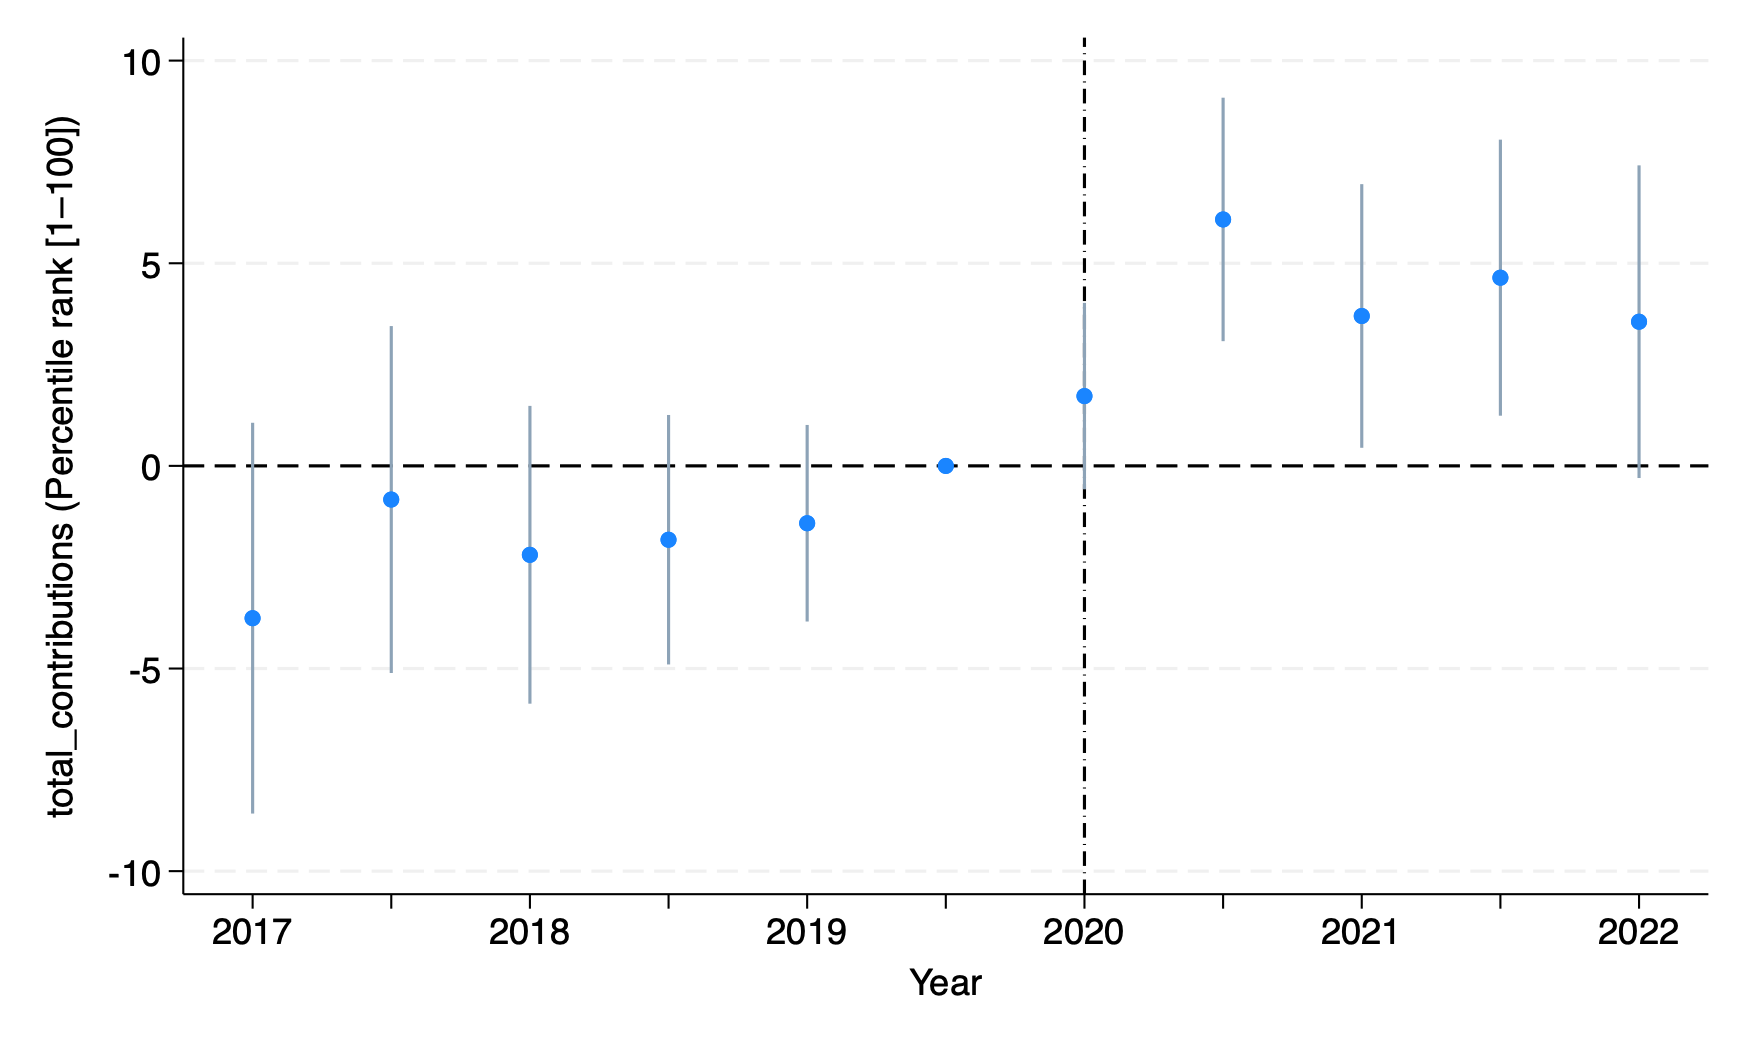
\includegraphics[width=0.9\textwidth]{\cleanedresultsdir/ols_total_contributions_q100.png}\\[2pt]
  \caption*{OLS – Total Contributions}
  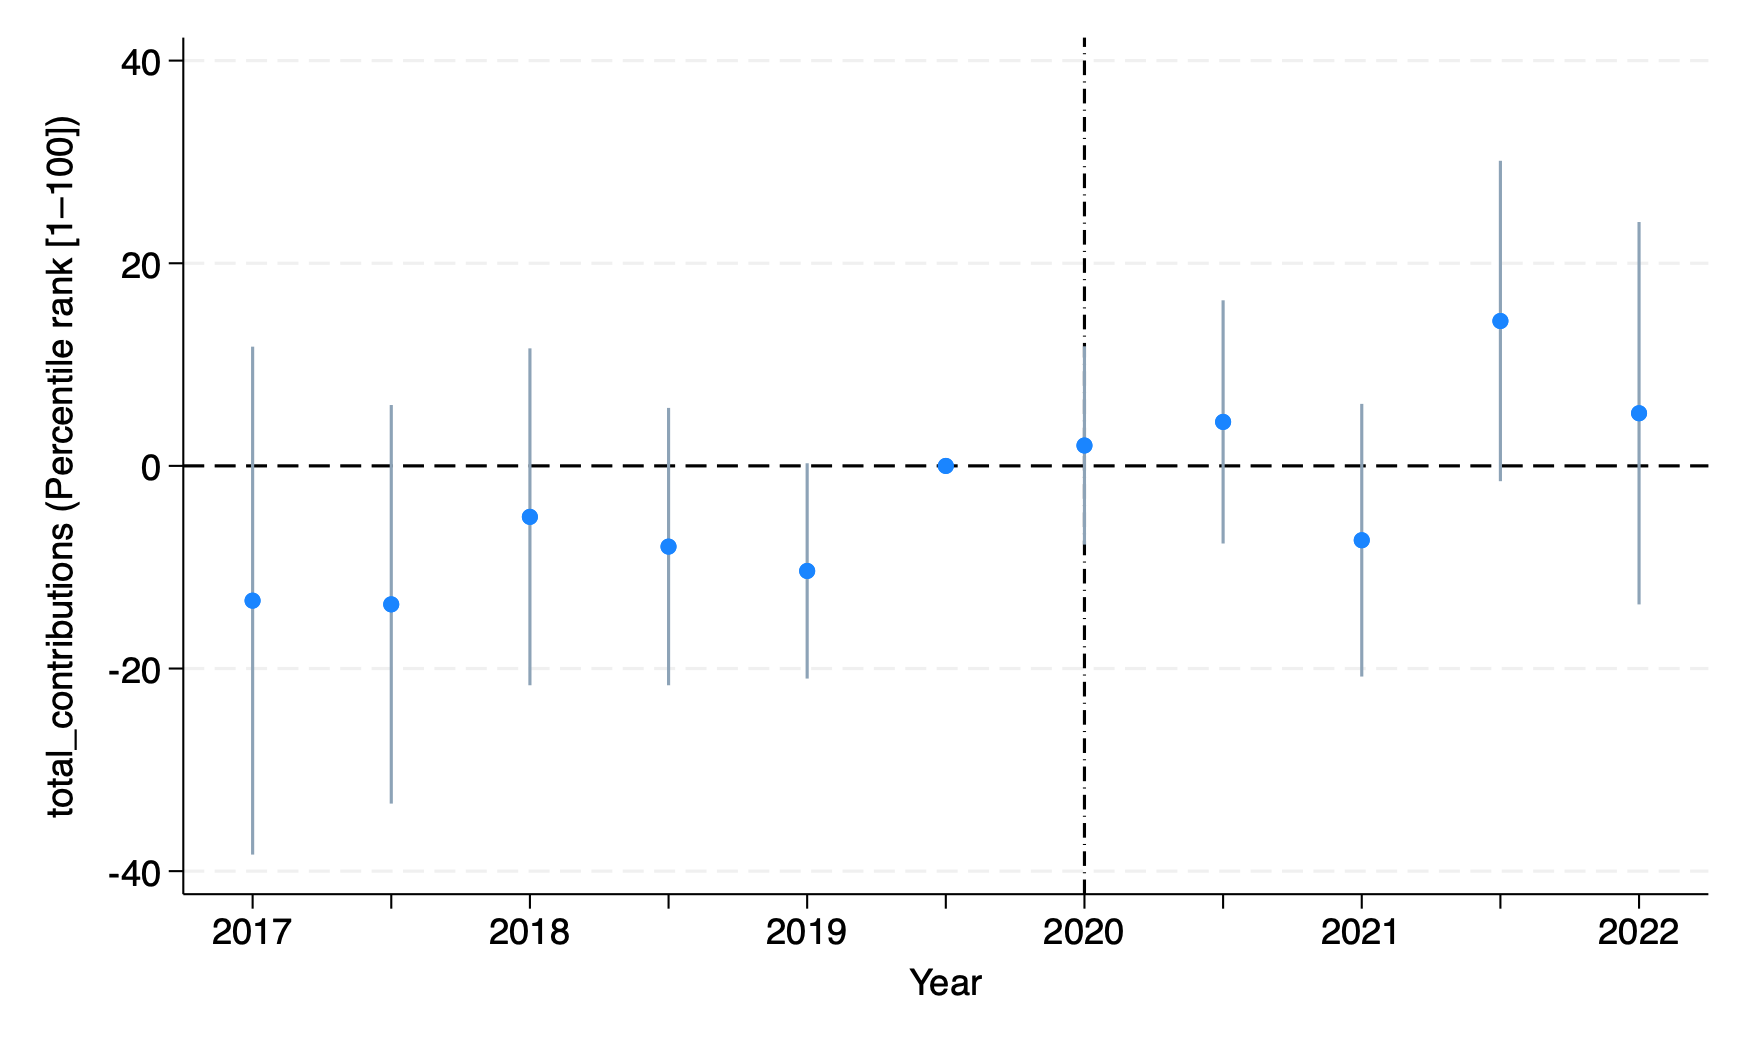
\includegraphics[width=0.9\textwidth]{\cleanedresultsdir/iv_total_contributions_q100.png}\\[2pt]
  \caption*{IV – Total Contributions}
\end{figure}

\clearpage

\begin{figure}[H]
  \centering
  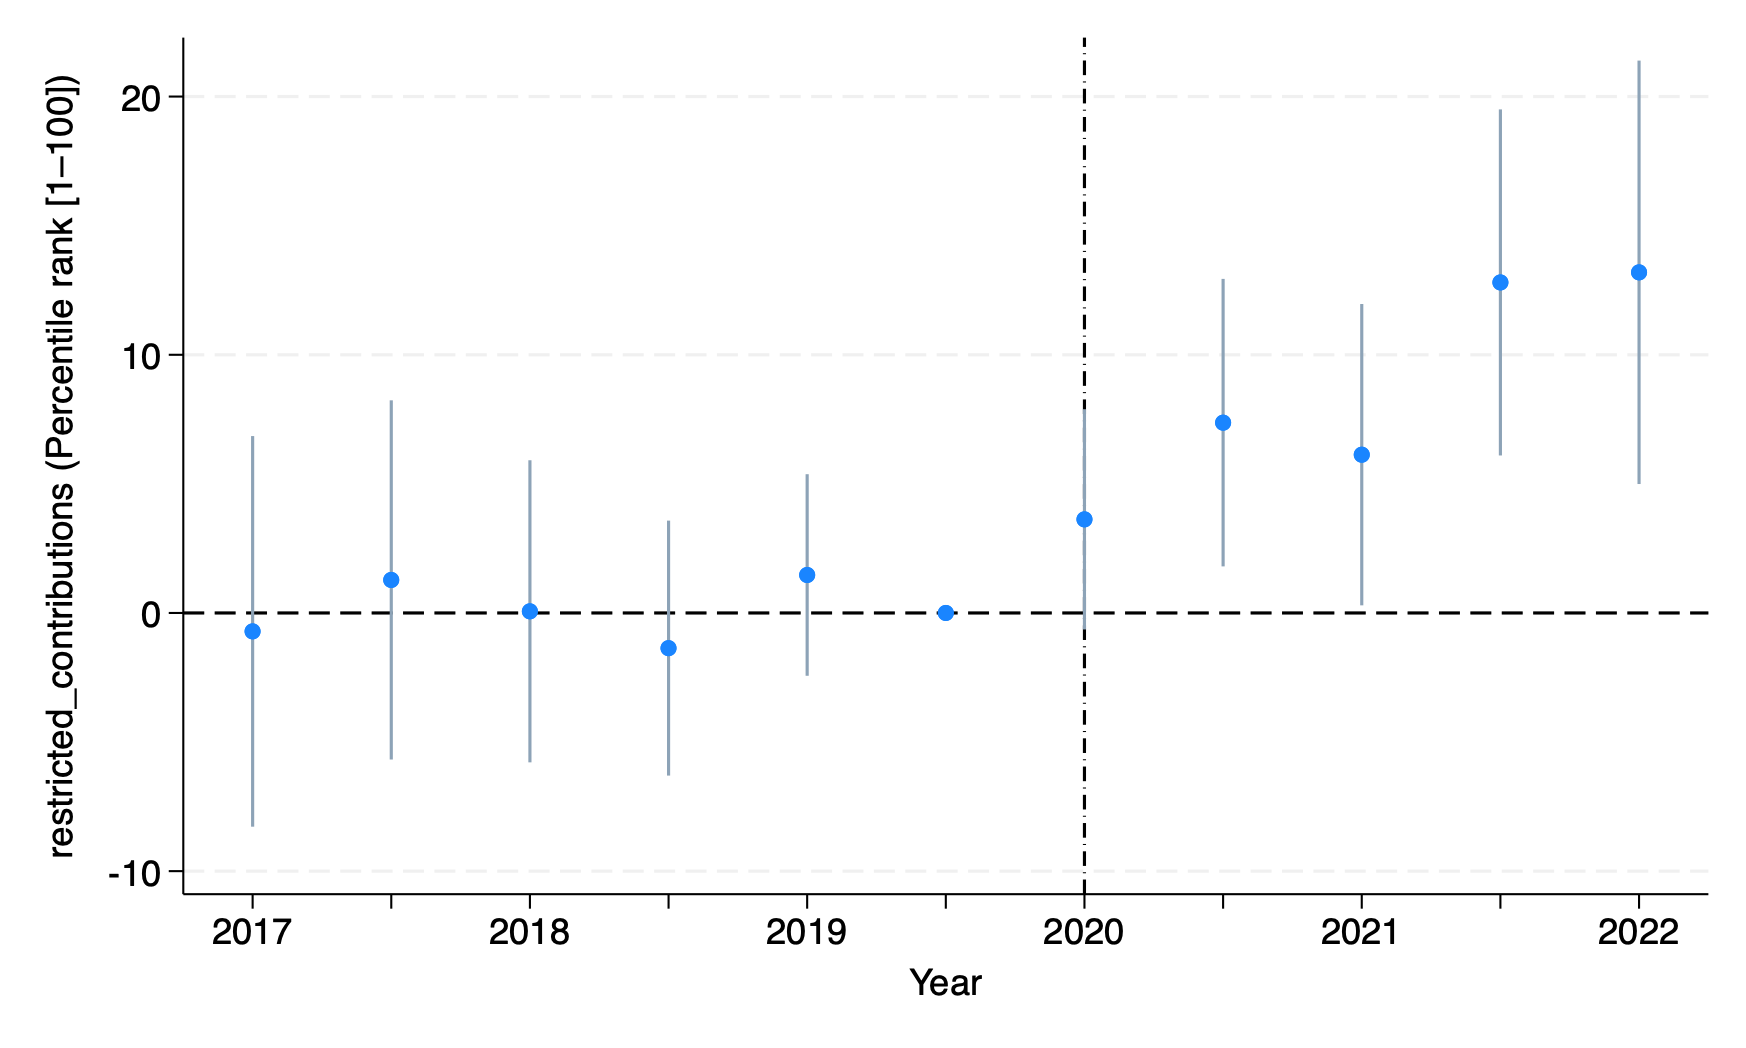
\includegraphics[width=0.9\textwidth]{\cleanedresultsdir/ols_restricted_contributions_q100.png}\\[2pt]
  \caption*{OLS – Restricted Contributions}
  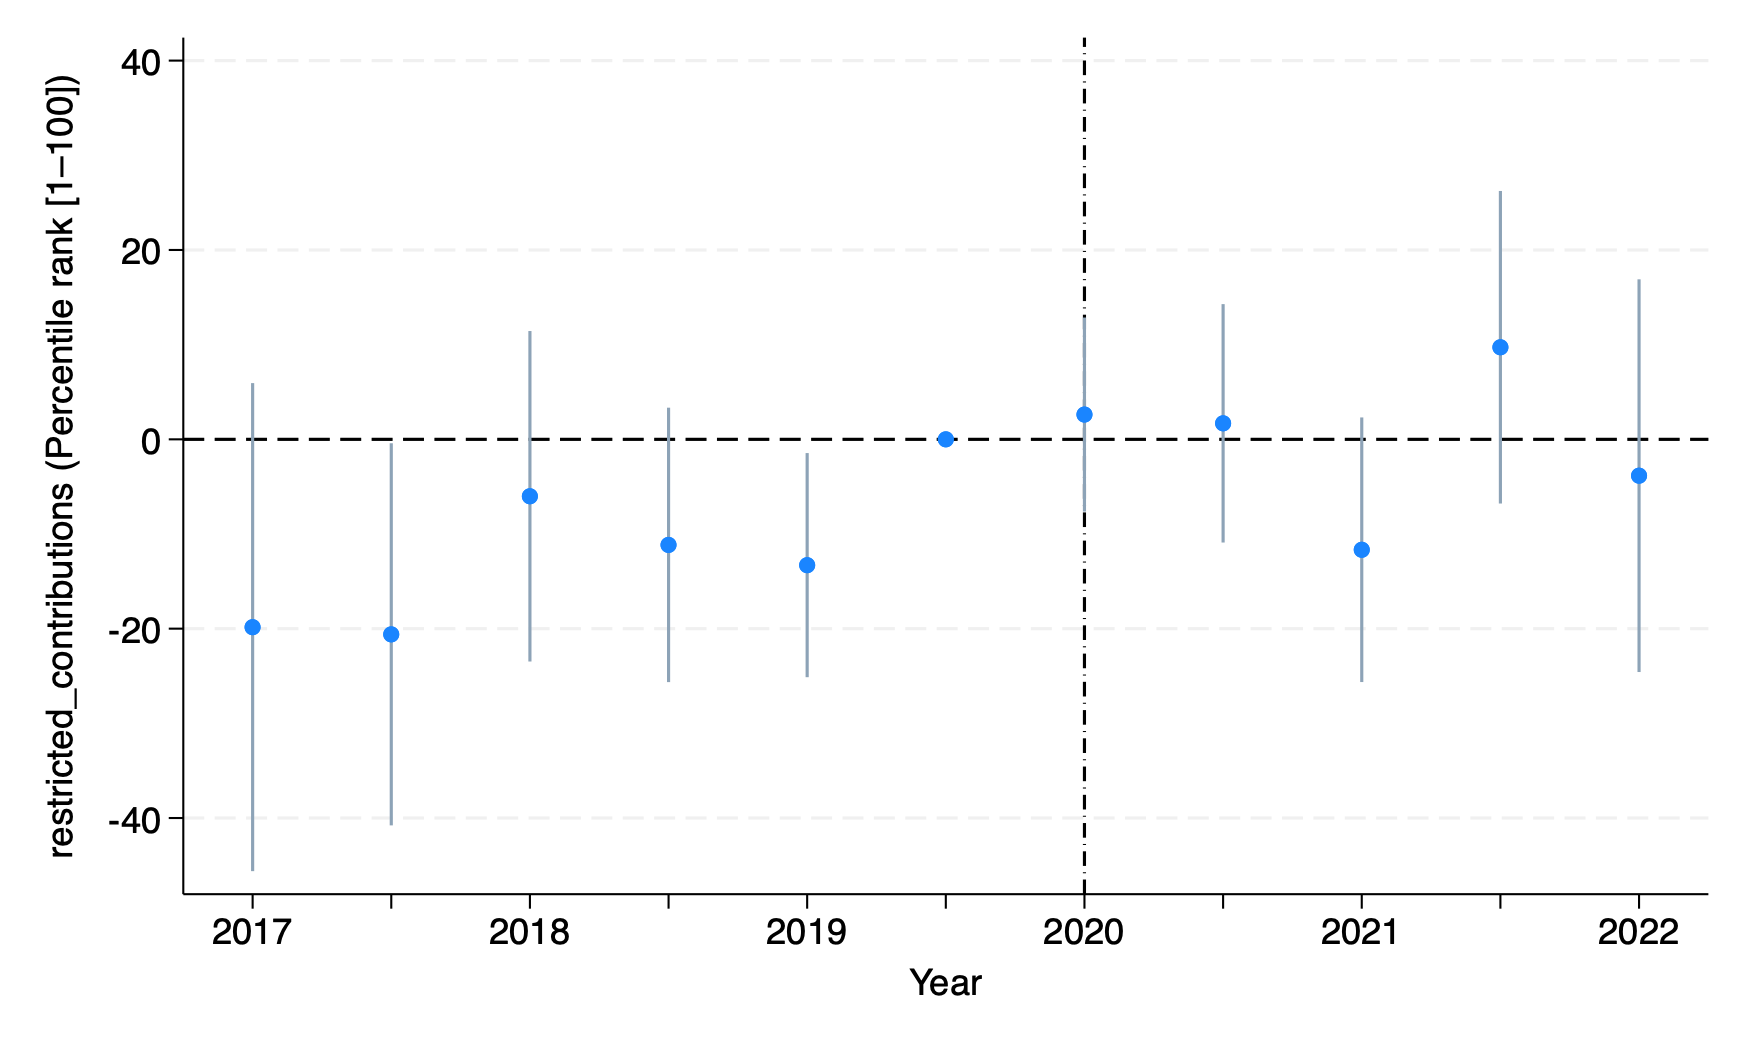
\includegraphics[width=0.9\textwidth]{\cleanedresultsdir/iv_restricted_contributions_q100.png}\\[2pt]
  \caption*{IV – Restricted Contributions}
\end{figure}

\clearpage

% ------------------------------------------------------------------
%  Firm-level outcomes
% ------------------------------------------------------------------

\begin{figure}[H]
  \centering
  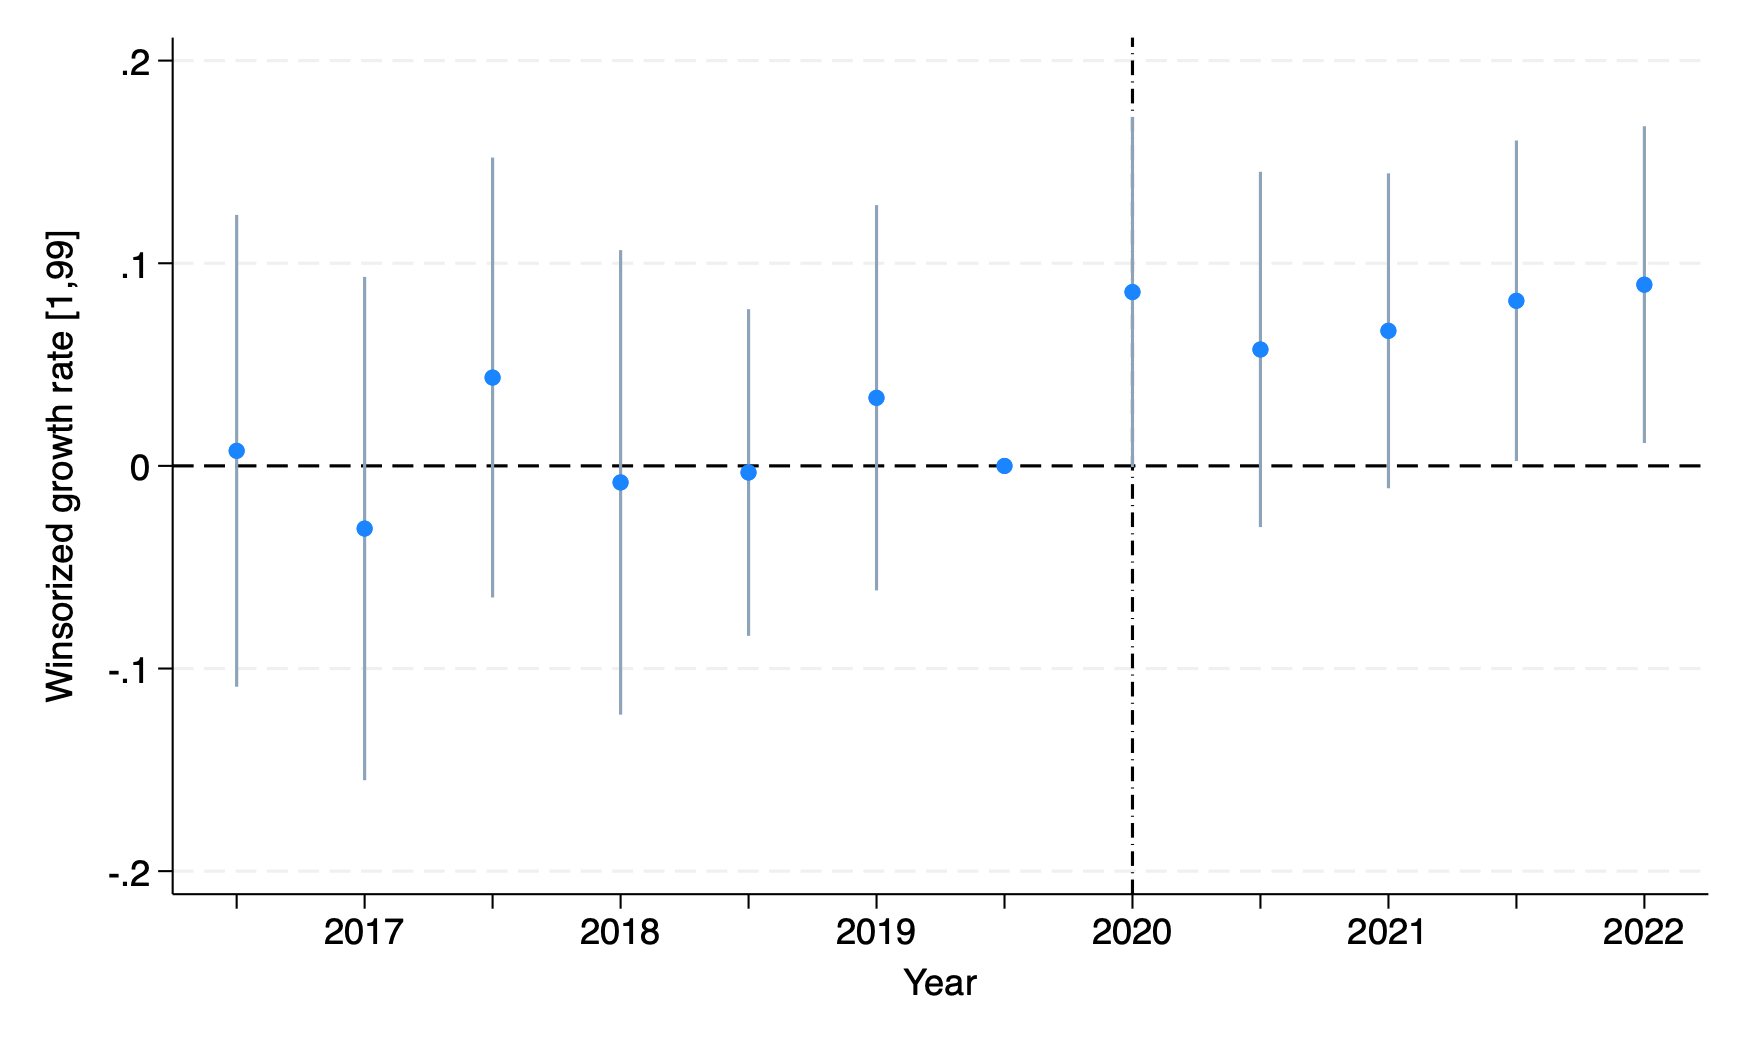
\includegraphics[width=0.9\textwidth]{\cleanedresultsdir/ols_growth_rate_we.png}\\[2pt]
  \caption*{OLS – Employment Growth}
  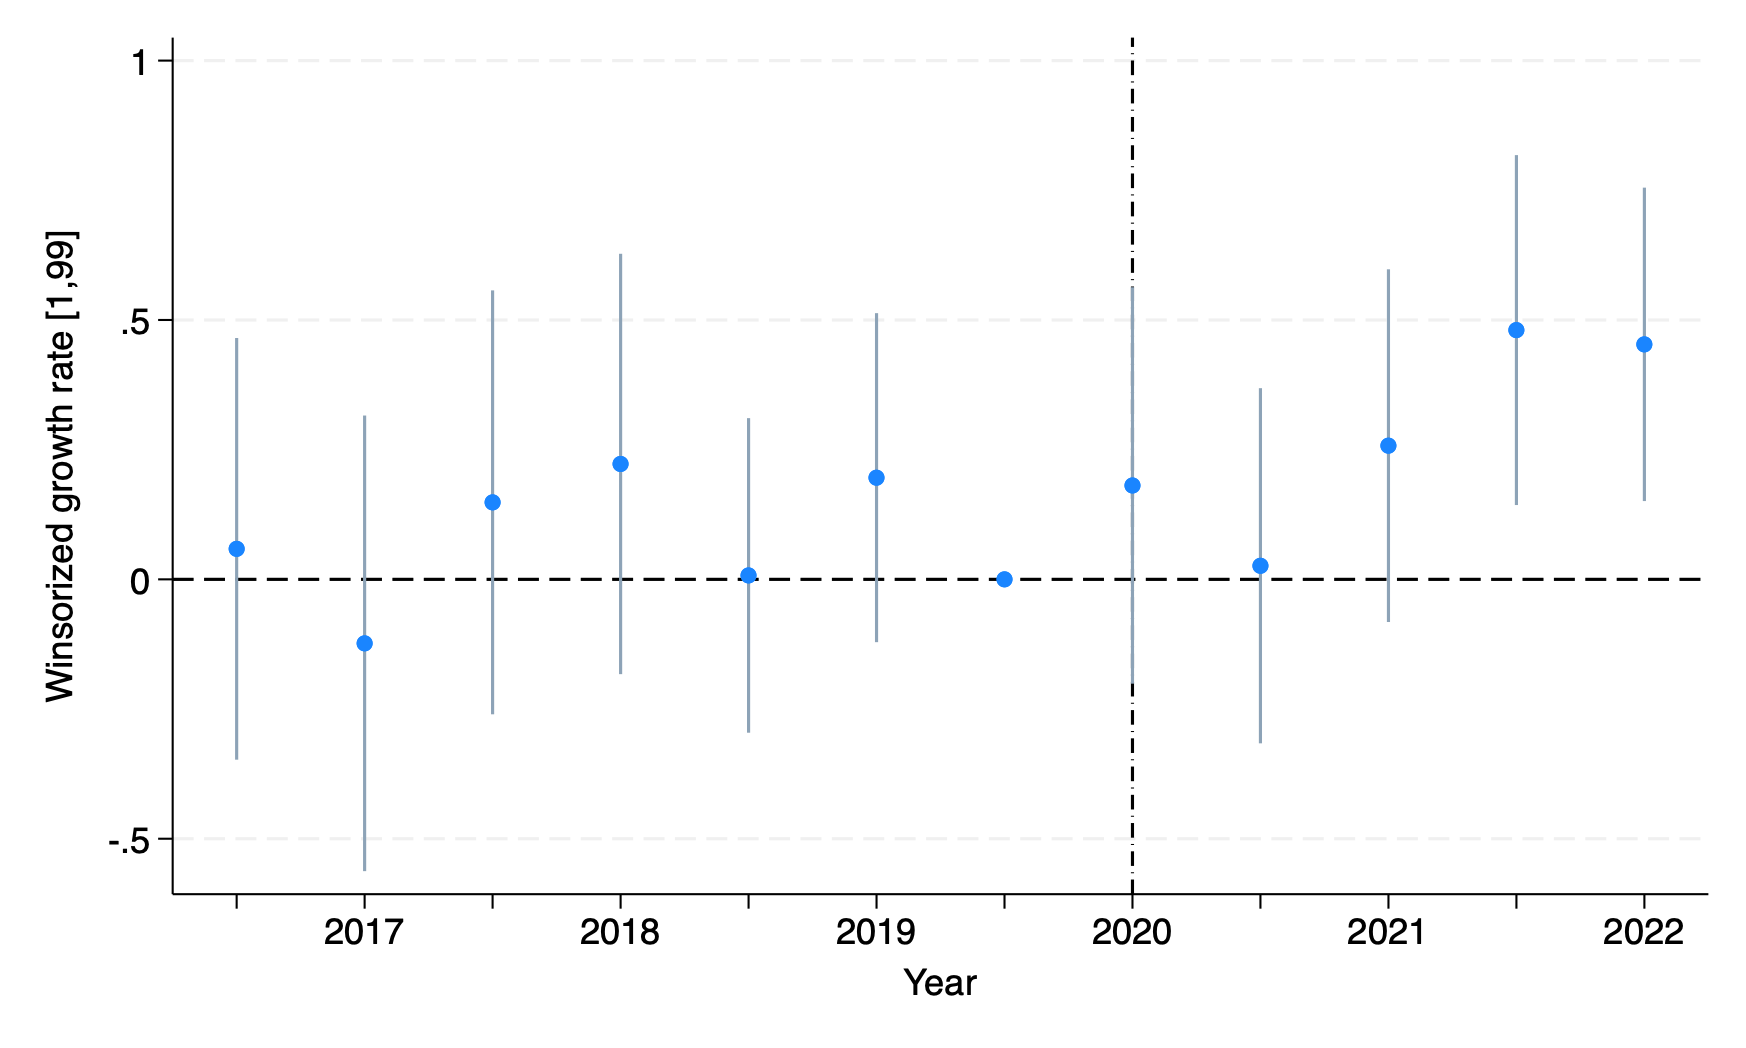
\includegraphics[width=0.9\textwidth]{\cleanedresultsdir/iv_growth_rate_we.png}\\[2pt]
  \caption*{IV – Employment Growth}
\end{figure}

\clearpage

\begin{figure}[H]
  \centering
  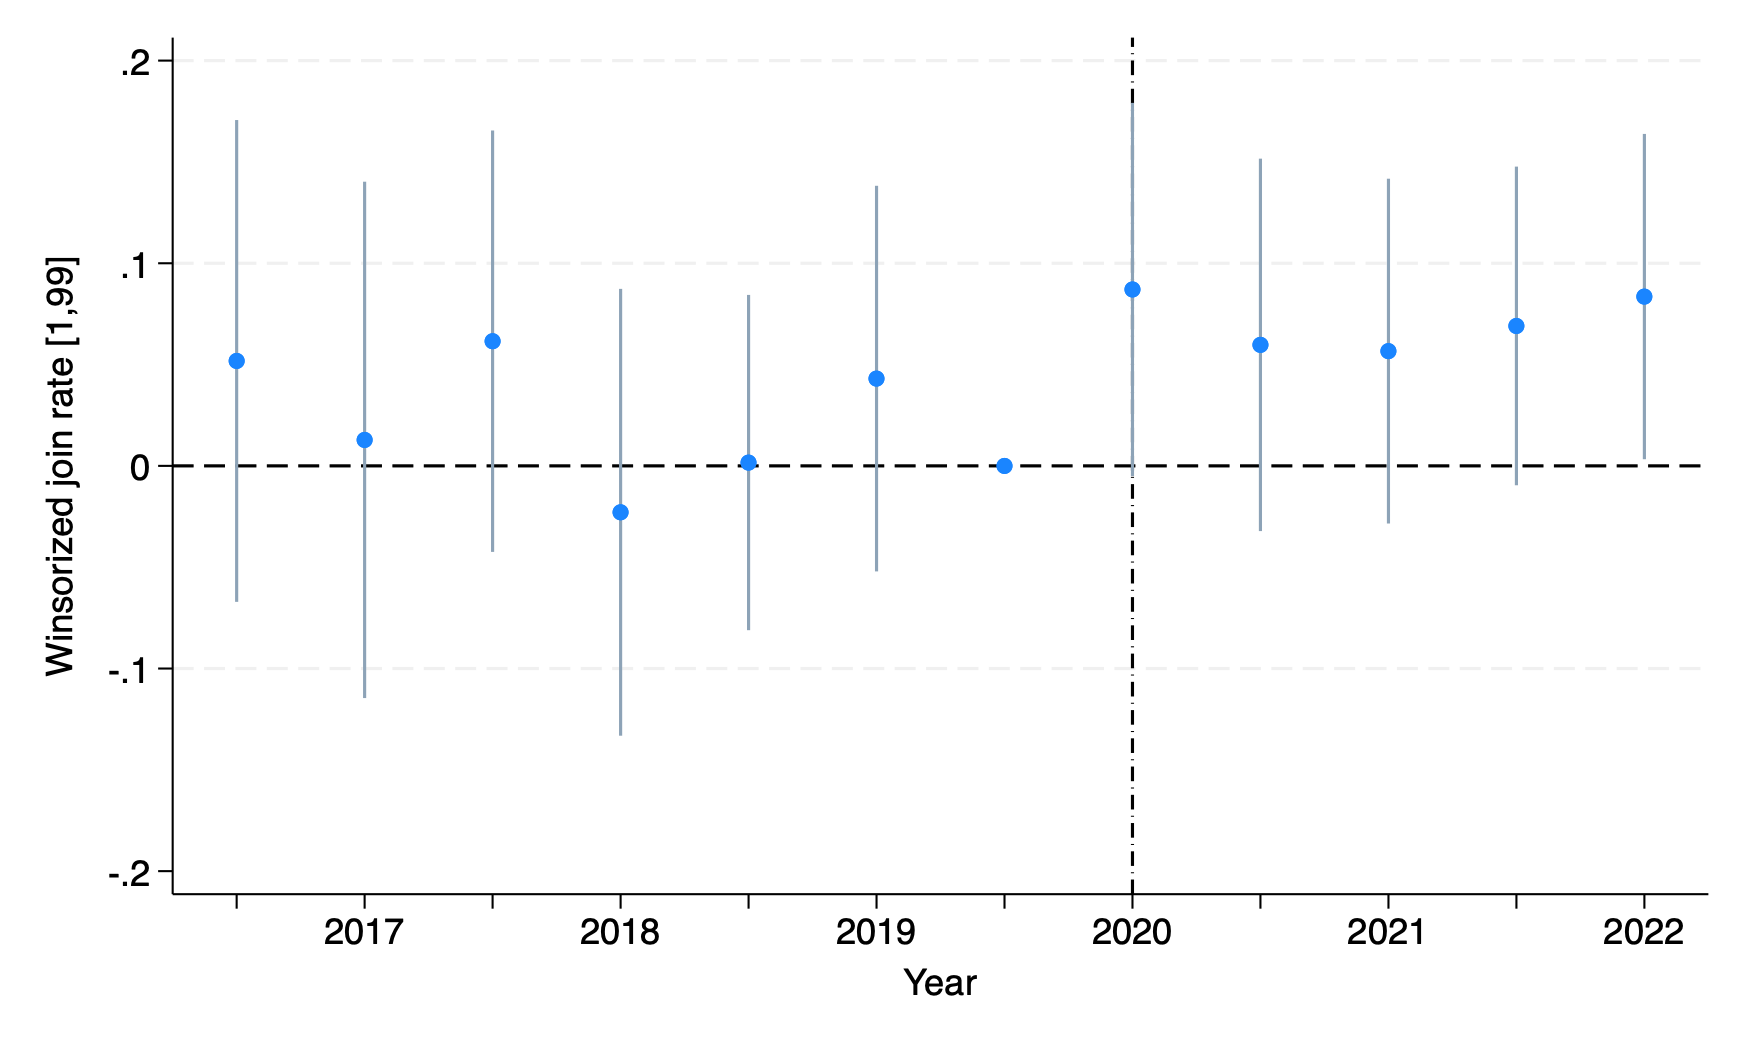
\includegraphics[width=0.9\textwidth]{\cleanedresultsdir/ols_join_rate_we.png}\\[2pt]
  \caption*{OLS – Join Rate}
  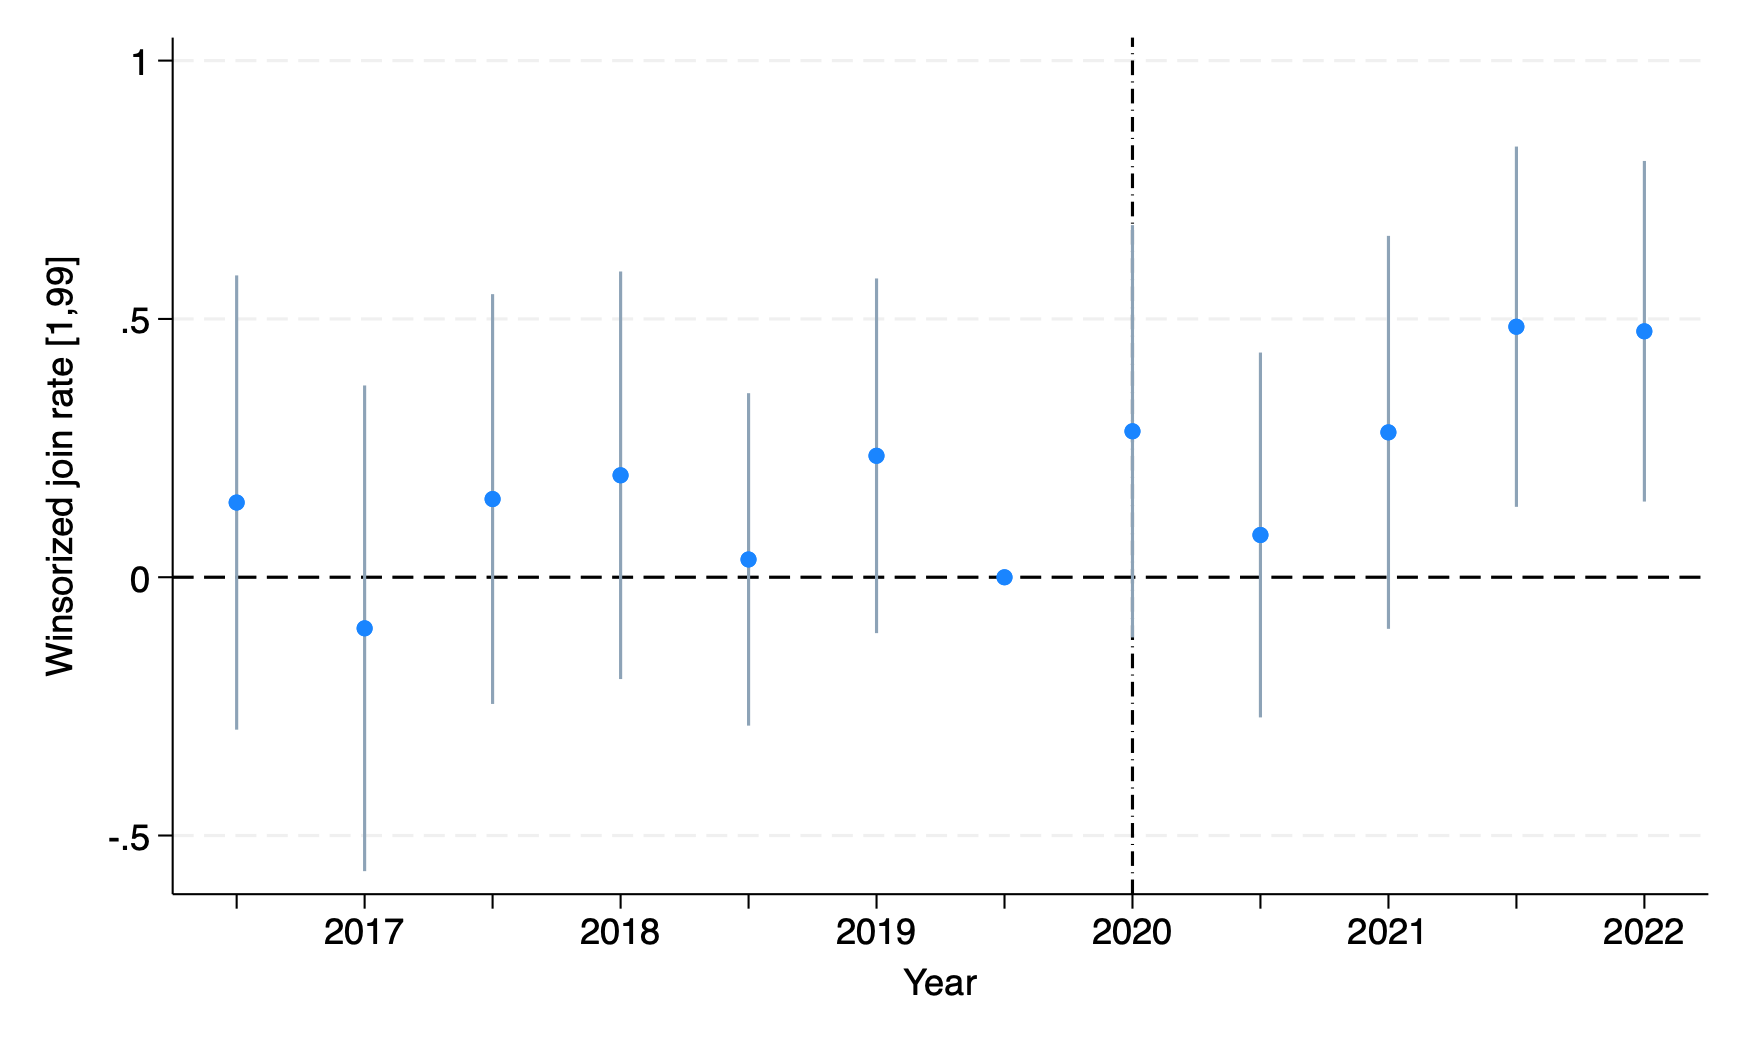
\includegraphics[width=0.9\textwidth]{\cleanedresultsdir/iv_join_rate_we.png}\\[2pt]
  \caption*{IV – Join Rate}
\end{figure}

\clearpage

\begin{figure}[H]
  \centering
  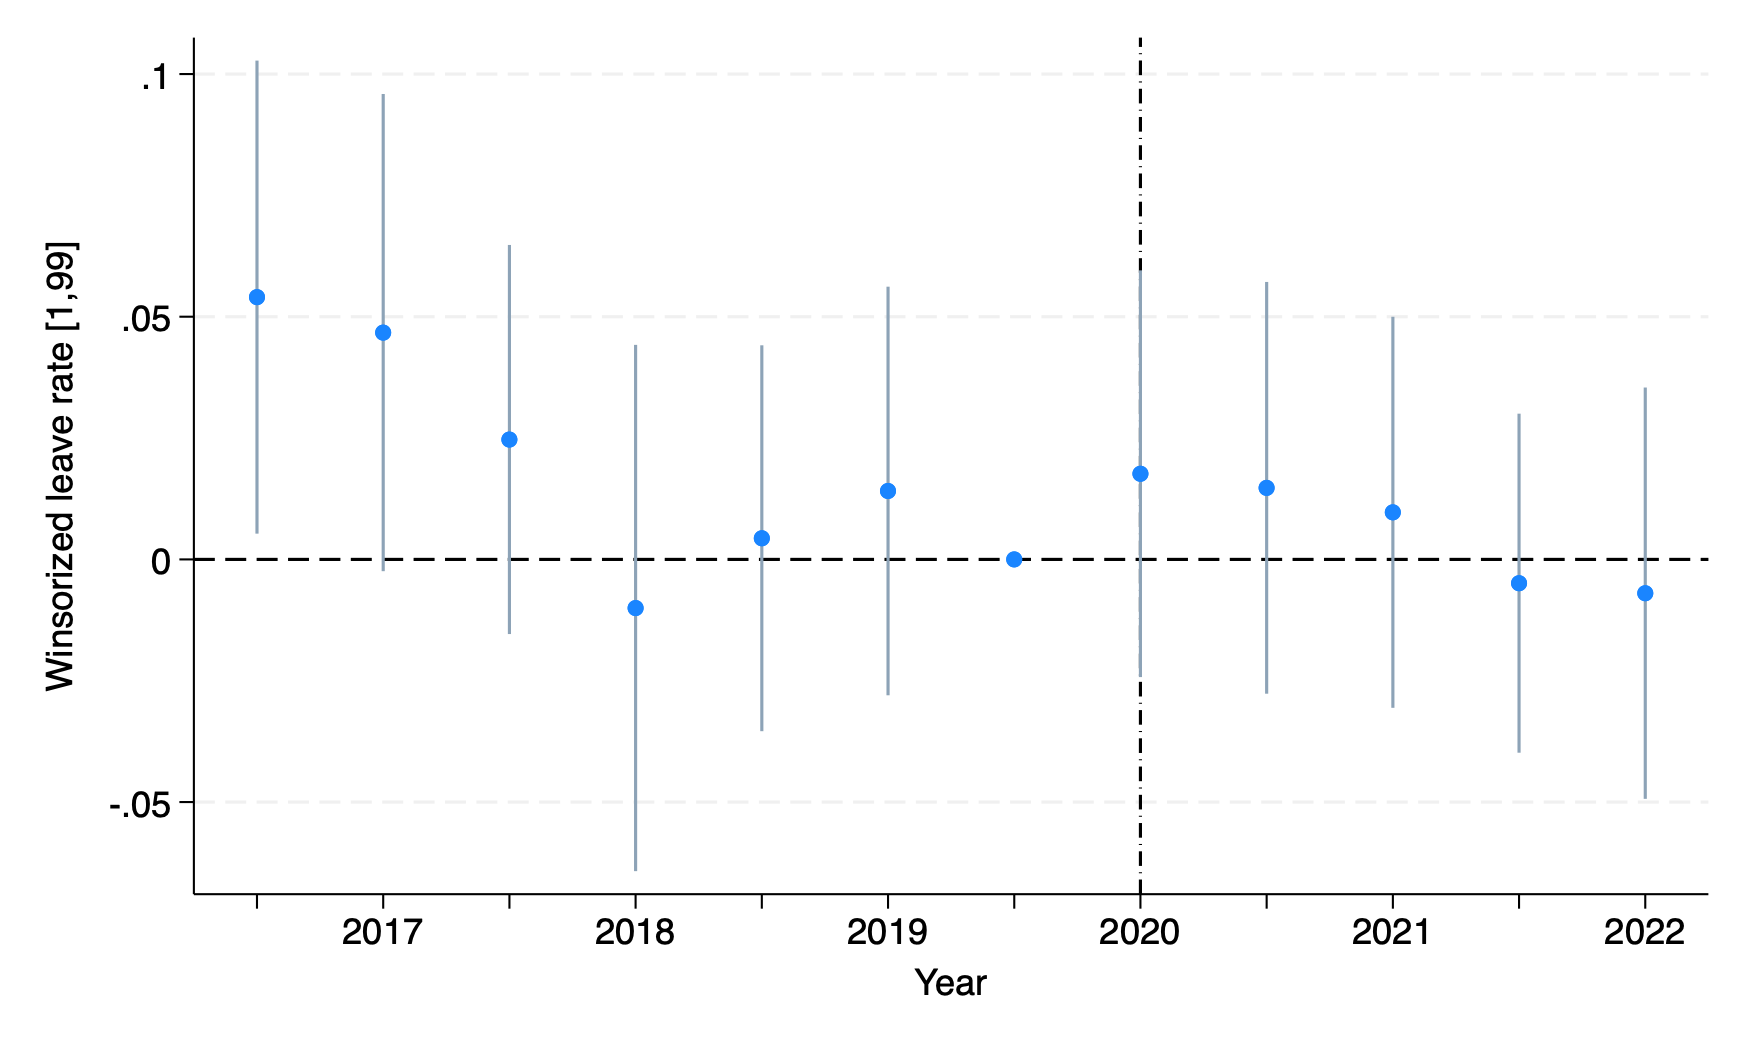
\includegraphics[width=0.9\textwidth]{\cleanedresultsdir/ols_leave_rate_we.png}\\[2pt]
  \caption*{OLS – Leave Rate}
  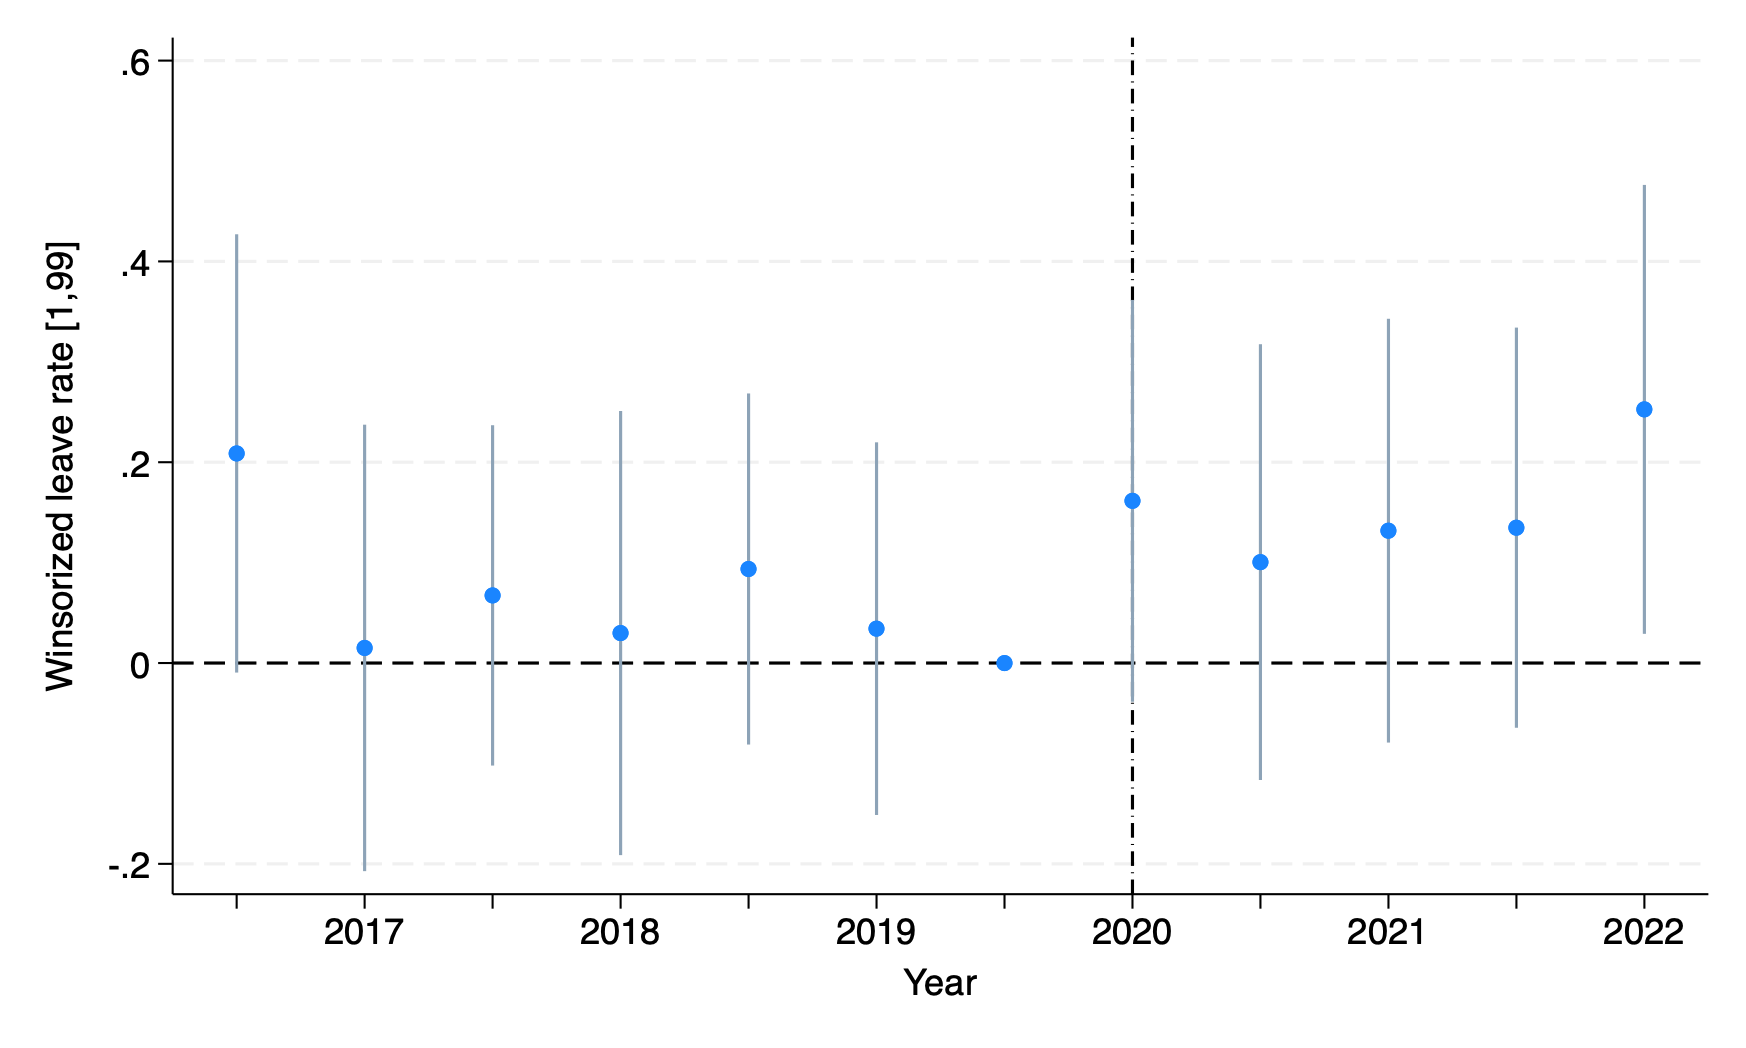
\includegraphics[width=0.9\textwidth]{\cleanedresultsdir/iv_leave_rate_we.png}\\[2pt]
  \caption*{IV – Leave Rate}
\end{figure}


\end{document}
